\documentclass{article}

% \usepackage{corl_2024} % Use this for the initial submission.
\usepackage[final]{corl_2024} % Uncomment for the camera-ready ``final'' version.
%\usepackage[preprint]{corl_2024} % Uncomment for pre-prints (e.g., arxiv); This is like ``final'', but will remove the CORL footnote.

\usepackage{amsmath, amsfonts}
\usepackage{amssymb}
\usepackage{mathtools}
\usepackage{multirow, makecell}

\usepackage{algorithmic}
\usepackage{algorithm}
\usepackage{array}
\usepackage[caption=false,font=normalsize,labelfont=sf,textfont=sf]{subfig}
\usepackage{textcomp}
\usepackage{stfloats}
\usepackage{url}
\usepackage{verbatim}
\usepackage{graphicx,import}
%\usepackage{cite}
\usepackage{color}
\usepackage{booktabs}
\usepackage{etoolbox}
\usepackage{bbm}
\usepackage{wrapfig}

% For coloring the tables
\usepackage[table]{xcolor}
\usepackage{pgf}



%% the rest of your preamble here
\newcommand\blfootnote[1]{%
  \begingroup
  \renewcommand\thefootnote{}\footnote{#1}%
  \addtocounter{footnote}{-1}%
  \endgroup
}







\newcommand\eva[1]{\textcolor{pink}{Eva: #1}}
\newcommand\toptile[1]{top_{#1}}
\newcommand\bottomtile[1]{bot_{#1}}
\newcommand\lefttile[1]{lef_{#1}}
\newcommand\righttile[1]{rig_{#1}}
\newcommand{\coms}{\xspace\scalebox{0.5}{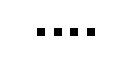
\begin{tikzpicture}\draw[dash pattern=on 3pt off 3pt, line width = 1mm ] (0,0) -- (0.8,0); \node at (0,-0.08) {}; \end{tikzpicture}}\xspace}
\newcommand{\moves}{\rightarrow}
\newcommand{\colorellipse}{orange!20!white}
\newcommand{\addCommunicationB}[1]
{
	\node[above right = 0.5mm and 4mm of #1, inner sep=0mm] (nb2) {B};
	\draw[tobehere,communication] (#1) -- (nb2);
}

\newcommand\setnodes{V}
\newcommand\basenode{B}
\newcommand{\sourcenode}{s}
\newcommand{\targetnode}{t}
\newcommand\USTCONN{USTCONN}
\newcommand\UCONN{UCONN}
\newcommand{\myundirectedgraphbounded}{\mathfrak G}
\newcommand{\myundirectedgraph}{\mathfrak G'}

\newcommand\pb[2]{${#1}_{#2}$~}

\newcommand\pbReach[1]{\pb{Reachability}{#1}}
\newcommand\pbBReach[1]{\pb{bReachability}{#1}}
\newcommand\pbCoverage[1]{\pb{Coverage}{#1}}
\newcommand\pbBCoverage[1]{\pb{bCoverage}{#1}}

\newcommand{\idDir}{dir}	% identifier for directed topological graph
\newcommand{\idNC}{nc}		% identifier for neighbor-communicable topological graph
\newcommand{\idSM}{sm}		% identifier for sight-moveable topological graph
\newcommand{\idCC}{cc}		% identifier for complete-communication topological graph
\newcommand{\idUnd}{und}		% identifier for complete-communication topological graph

\newcommand{\pbReachDir}{\pbReach{\idDir}}
\newcommand{\pbBReachDir}{\pbBReach{\idDir}}
\newcommand{\pbCoverageDir}{\pbCoverage{\idDir}}
\newcommand{\pbBCoverageDir}{\pbBCoverage{\idDir}}

\newcommand{\pbReachNC}{\pbReach{\idNC}}
\newcommand{\pbBReachNC}{\pbBReach{\idNC}}
\newcommand{\pbCoverageNC}{\pbCoverage{\idNC}}
\newcommand{\pbBCoverageNC}{\pbBCoverage{\idNC}}

\newcommand{\pbReachSM}{\pbReach{\idSM}}
\newcommand{\pbBReachSM}{\pbBReach{\idSM}}
\newcommand{\pbCoverageSM}{\pbCoverage{\idSM}}
\newcommand{\pbBCoverageSM}{\pbBCoverage{\idSM}}

\newcommand{\pbReachCC}{\pbReach{\idCC}}
\newcommand{\pbBReachCC}{\pbBReach{\idCC}}
\newcommand{\pbCoverageCC}{\pbCoverage{\idCC}}
\newcommand{\pbBCoverageCC}{\pbBCoverage{\idCC}}

\newcommand{\pbReachUnd}{\pbReach{\idUnd}}
\newcommand{\pbBReachUnd}{\pbBReach{\idUnd}}
\newcommand{\pbCoverageUnd}{\pbCoverage{\idUnd}}
\newcommand{\pbBCoverageUnd}{\pbBCoverage{\idUnd}}

\newtheorem{theorem}{Theorem}
\newtheorem{fact}[theorem]{Fact}
\newtheorem{definition}[theorem]{Definition}
\newtheorem{proposition}[theorem]{Proposition}
%\newtheorem{proof}{Proof}
\newtheorem{lemma}[theorem]{Lemma}

\tikzstyle{copyofG} = [fill=gray!20!white, draw=none, rounded corners=8pt]
\tikzstyle{communication} = [dash pattern=on 1pt off 1pt] %[line cap=rect, dot diameter=1pt, dot spacing=2pt, dots] %[dash pattern=on 2pt off 2pt on \the\pgflinewidth off 2pt]
\tikzstyle{tobehere} = [color=blue!50!white]
\newcommand\set[1]{\{#1\}}
\newcommand\suchthat{\mid}
\newcommand{\nbdrones}{n}

\newcommand{\booleanvariablegeneric}{{x}}
\newcommand{\clausegeneric}{\mathsf{c}}

\newcommand{\ok}{\includegraphics[height=2mm]{check.png}}
\newcommand{\imgDrone}{\includegraphics[height=2mm]{drone_black.png}}

\usetikzlibrary{decorations.pathmorphing}
\usetikzlibrary{decorations.pathreplacing}
\usetikzlibrary{arrows}
\usetikzlibrary{positioning}

\makeatletter
\tikzset{
	dot diameter/.store in=\dot@diameter,
	dot diameter=3pt,
	dot spacing/.store in=\dot@spacing,
	dot spacing=10pt,
	dots/.style={
		line width=\dot@diameter,
		line cap=round,
		dash pattern=on 0pt off \dot@spacing
	}
}
\makeatother

%%% Local Variables:
%%% mode: latex
%%% TeX-master: "main"
%%% End:


\title{Scaling Safe Multi-Agent Control for Signal Temporal Logic Specifications}

% The \author macro works with any number of authors. There are two
% commands used to separate the names and addresses of multiple
% authors: \And and \AND.
%
% Using \And between authors leaves it to LaTeX to determine where to
% break the lines. Using \AND forces a line break at that point. So,
% if LaTeX puts 3 of 4 authors names on the first line, and the last
% on the second line, try using \AND instead of \And before the third
% author name.

% NOTE: authors will be visible only in the camera-ready and preprint versions (i.e., when using the option 'final' or 'preprint'). 
% 	For the initial submission the authors will be anonymized.

\author{
      Joe Eappen, Zikang Xiong, Dipam Patel, Aniket Bera, Suresh Jagannathan\\
  % \textdagger Department of ECE, *Department of CS\\
  Purdue University \\
  West Lafayette, IN 47907, United States\\
  \texttt{\{jeappen,xiong84,dipam,aniketbera,sjaganna\}@purdue.edu}
  %% \AND
  %% Coauthor \\
  %% Affiliation \\
  %% Address \\
  %% \texttt{email} \\
  %% \And
  %% Coauthor \\
  %% Affiliation \\
  %% Address \\
  %% \texttt{email} \\
  %% \And
  %% Coauthor \\
  %% Affiliation \\
  %% Address \\
  %% \texttt{email} \\
}
\begin{document}
	
%\markboth{IEEE Robotics and Automation Letters}%
%{Shell \MakeLowercase{\textit{et al.}}: A Sample Article Using IEEEtran.cls for IEEE Journals}

%\IEEEpubid{0000--0000/00\$00.00~\copyright~2021 IEEE}
\maketitle

%===============================================================================

\begin{abstract}
  % We present a scalable approach to multi-agent control for Signal Temporal Logic (STL) specifications. 
  % We propose a novel method that combines a multi-agent collision avoidance controller
  % with a Graph Neural Network (GNN) based planner trained on an STL objective
  % to generate safe and efficient plans for multiple agents. 
  % Our approach uses an end-to-end differentiable technique with the STL robustness metric to optimize for the satisfaction of complex temporal specifications given a controller with multi-agent collision avoidance capabilities.
  % We demonstrate the effectiveness of our approach on a range of STL specifications and show that our method can scale to a large number of agents and complex specifications.
  % Our experiments show that our approach outperforms existing methods that use a purely single-agent view or a state-of-the-art MILP-based planner in terms of scalability and performance.
%  \zk{tweaked the order of sentences a bit}
Existing methods for safe multi-agent control using logic specifications like Signal Temporal Logic (STL) often face scalability issues. This is because they rely either on single-agent perspectives or on Mixed Integer Linear Programming (MILP)-based planners, which are complex to optimize. These methods have proven to be computationally expensive and inefficient when dealing with a large number of agents. To address these limitations, we present a new scalable approach to multi-agent control in this setting. Our method treats the relationships between agents using a graph structure rather than in terms of a single-agent perspective. Moreover, it combines a multi-agent collision avoidance controller with a Graph Neural Network (GNN) based planner, models the system in a decentralized fashion, and trains on STL-based objectives to generate safe and efficient plans for multiple agents, thereby optimizing the satisfaction of complex temporal specifications while also facilitating multi-agent collision avoidance. Our experiments show that our approach significantly outperforms existing methods that use a state-of-the-art MILP-based planner in terms of scalability and performance.
  \end{abstract}

% TDLR: Graphical Neural Networks (GNNs) can help scale Specification-driven control on Multi-agent systems beyond existing Mixed Integer Linear Programming (MILP)-based planners.

% Two or three meaningful keywords should be added here
%\begin{IEEEkeywords}
%Multi-Robot Systems, Path Planning for Multiple Mobile Robots or Agents, Collision Avoidance, Hybrid Logical/Dynamical Planning and Verification, Deep Learning Methods
%\end{IEEEkeywords}

\keywords{Multi-Robot Systems, Path Planning for Multiple Mobile Robots, Collision Avoidance, Specification-Guided Learning, Deep Learning Methods} 

%===============================================================================


%{\bf \large{Some references}}\\
%\begin{itemize}
%    \item\cite{Wang2015} Optimal control for epidemic routing of two files with different priorities in Delay Tolerant Networks
%  A Multi-Layer Swarm Control Model for Information Propagation and Multi-Tasking 2019 ACC Fuming Zhang
%\end{itemize}
%Outline - 
%The problem is defined as controlling the performance of a network composed of mobile robots by controlling the the individual performance (define performance) of each of the node.

%The multi-robot system has an architecture that can be described by a graph determined by their positions and interactions. The topology and the features (define features) of the interactions together delivers the performance (of information propagation, routing, etc.) of a network.

%Uncertainty brings in randomness. Exsting work only considers certain stochasticity - whether a link is there or not. There are other issues to be consider. e.g. - The distances between different pairs of robots only only defined the topology, which specifies who can talk with who, but also how good they are communicating. The transmission quality can be described by a transmission rate, which converged the completion of transmission on one link into a Poisson process (that the completion is seen as an event).

%Existing graph theory tools can handle either a static graph or a time-varying graph with known dynamics (or random graphs). When the uncertainty disrupts the dynamics, existing tools all fail. We need new tools analyzing graphs that :1) with stochasticity in diffrent ~ , 2) with structues / patterns that we can leverage.

%So that we can deliver control schemes that can guarantee/optimize the performance of the network in a decentralized fashion.


%\subsection{Existing results}
%Li found a way of determining the most important links considering the chronological order.

%\subsection{Challenge}
%(maybe future work - If we want to improve the transmission quality, we essentially want to move that pair of robots close to each other.

%However, moving robots will affect the relative position to other robots. 

%Improving transmission rate all around may cause conglomeration.

%We may want to find a way of moving robots to improve the topology / transmission but not to cause conglomeration.)

%\subsection{Approach}

%\paragraph{Stage I:}
%The topology of the communication network is fixed. Any robot improving its communication quality with one of its neighbours will suffer from a decreased communication quality with other neighbors. 

%Model - Fixed topology, robot $i$ has $d_1$ neighbors, the delivery of a piece of message along a communication link is modeled as a Poisson process, each communication channel is associated with a parameter $\lambda_{ij}$ determining the Poisson process. We have $\sum_{\forall j} \lambda_{ij} = 1$.

%Aim - control each node's distribution of $\lambda$ to optimize the performance of the system.

%To be added - the model of information resources?

%\paragraph{Stage II:}
%The robots are moving on a 1-D or 2-D space that moving closer towards one neighbor with risk distancing itself with other neighbors.

%The 'perimeter' nodes are fixed.

%Communication qualify is related to the distance between the pair of robots. 

We are interested in leveraging spatio-temporal sensing capabilities of robotic teams to explore or monitor large-scale complex environments
(\textit{e.g.,} forests, oceans, and underground caves and tunnels \cite{breitenmoser2010voronoi,cassandras2016smart,gusrialdi2008voronoi,wei2018,yu2019synchronous}).
%\xyucomment{I mean 'deliver the tasks'. I edit the sentence accordingly. Thanks!}
While individual robots can each monitor or explore limited regions, a team of them can efficiently cover larger areas.  Naturally, individual robots in swarms are expected
to exchange information and make certain decisions based on the information gathered by itself and received from other robots \cite{hsieh2008decentralized,moarref2020automated}.
It is, therefore, essential for any robot to be able to
transmit its gathered data to others in the team. 

As the demand of information transmission can emerge between any pair of nodes, we use a propagation model to study the efficiency of the connectivity of the whole team. 
In such models, robots are represented as nodes of a graph,
and interactions 
%(\textit{i.e.} communication)
between nodes are represented by edges.
%The nodes and the edges together form a network.
At the beginning of a propagation, the nodes 
%(\textit{i.e.} robots) 
are considered as `non-informed', and will be `informed’ by the information propagated through the graph. A faster convergence of all nodes into the status of `informed' indicates a more \textit{efficiently connected} network. 
Existing works abstract the propagation of information from any individual agent to the rest of the team as compartmental models \cite{huang2006information,khelil2002epidemic,zanette2002dynamics}, which are also broadly used in modeling the spread of an infectious diseases \cite{brauer2008compartmental}.
%In such models, robots are represented as nodes of a graph,
%and interactions 
%(\textit{i.e.} communication)
%between nodes are represented by edges.
%The nodes and the edges together form a network.
% The nodes 
% %(\textit{i.e.} robots) 
% are labeled according to their status of whether the robots are `informed’ by the information propagated through the swarm.
The flow of the nodes from one compartment to another
%(\textit{i.e.} uninformed robots get `informed’ with the information.)
occurs when active links exist between robots that are
`informed’ and `non-informed’ %the information 
(\textit{i.e.,} 
only `informed' robots %carrying the information 
can transmit the information to `non-informed' ones).%robots that are not yet informed). 


%\thales{However, epidemic models often operate under the assumption that the networks are static and deterministic, so that the flow between compartments can be analyzed with ordinary differential equations \cite{}. In reality, neither human contacts nor robots working in communication challenging environments can guarantee such consistent connectivity in large-scale networks. The classic compartmental-models-based control strategies for such networks also focus on the statistical behavior of the nodes, ignoring the topology of the networks. The analysis and solutions are, therefore, generally valid with giant node numbers reaching thermodynamic limits \cite{}. } 


However, compartmental models often focus on the statistical behavior of the nodes, overlooking the capabilities of the \textit{individual-level} decision making that may impact the network's performance.
%\xyucomment{I commented out this paragraph and edit it as a couple of bridge sentences. }
Recent works in robotics have noticed and embraced the potential of controlling individual robots so that the performance of the whole network (\textit{i.e.,} the transmission rates, if a propagation model is considered,) can be impacted or improved. %swarm can jointly achieve the desired status. 
The topology of networks was analyzed in \cite{Preciado2014} and control strategies were proposed to identify 
and isolate the nodes that have a higher impact on
the propagation process. The design of {\it time-varying} networks where robots leverage their mobility to move into each other's communication ranges to form and maintain temporal communication links has been addressed in  \cite{hollinger2012multirobot,khodayi2019distributed,yu2020synthesis}. Information can be propagated in such networks by relying on time-respect routing paths formed by a sequence chronologically ordered temporal links \cite{yu2020synthesis}. 
Nonetheless, such approaches still require thorough and perfect knowledge of the network's topology and the robots' ability to maintain active links and requires robots to execute their motion plans precisely both in time and space. As such, the resulting networks lack robustness to uncertainties in link formation timings that may result from errors in motion plan execution due to localization errors and/or actuation uncertainties.

%\thales{Stochastic models, such as networks based on percolation theory concepts \cite{}, have also been introduced in works in epidemiology in recent years to carry out a more realistic analysis. Percolation theory assumes a growing collection of edges between nodes. When the addition of edges fits a stochastic process, the growing graphs yielded are modeled as Erd\"os–R\'enyi networks, and have been well studied in the field of random graphs \cite{}. Noticed that such stochastic models focus on a random \textit{existence} of edges on a graph, echoing the assumption of Canadian Traveler Problems, in which the graphs are partially visible, and the edges are randomly blocked \cite{}. }

%Real-world communication networks synthesized in robot 
%swarms face uncertainties causing stochastic performance
%of the networks.
%that can not always be directly addressed by existing graph theory tools. 
Existing stochastic graph models focus on random changes in a network's topology centered around random creation and removal of edges within a graph. For example, the Canadian Traveller Problem assumes partially visible graphs where edges randomly appear and disappear \cite{bar1991canadian,nikolova2008route}.
For time-varying networks,
\cite{knizhnik2022flow,shen2022topology} assumed that any temporal link
may suffer from deviations from
its scheduled timing due to the uncertain arrival time of one robot into another robot’s communication range.
%\xyucomment{I commented out the original paragraph and edit the following graph as shown in blue. }
%Consider robot swarms moving in challenging environments
%with network topology changing over time.
%Any temporal link that occurs and disappears in such a network may suffer from deviations in its scheduled timing \cite{ACC2022} due to the uncertain arrival time of one robot into another robot’s communication range \cite{ICRA 2022}.
Information routing or propagation planned for such networks may experience severe delays if subsequent links along a routing path appear out of chronological order in the presence of link formation uncertainties resulting from uncertainties in robot motions \cite{yu2020synthesis}.  These challenges are addressed in \cite{shen2022topology} for networks with periodically time-varying interconnection topologies.  Control strategies to `fix’ nodes with 
higher impact on the whole network’s performance were also proposed in \cite{shen2022topology} similar in spirit to those presented in \cite{Preciado2014}.

In the Canadian Traveler Problems and \cite{shen2022topology}, messages are assumed to be transmitted instantaneously between nodes whenever a link appears. As such, the resulting strategies are solely based on the \textit{existence} of an available link between a certain pair of robots at a certain time point. When the time to transmit a message is non-trivial, the question goes beyond whether the information can be transmitted or not and must consider the quality of the transmission (\textit{e.g.,} safe, fast, confident). Consider a pair of robots flying through a Poisson forest maintaining a communication link that requires line-of-sight (LOS). The randomly distributed obstacles may intermittently disrupt the LOS between the robots causing randomized delay in the completion of the information transmission task. In these situations, it becomes difficult to determine whether a robot \textit{is} informed or not at a given time point which then impacts the robots ability to plan subsequent actions.

In this paper, we aim to develop receding horizon control schemes that allows individual robots to re-direct their transmission resources 
(\textit{e.g.,} time, power) to different neighboring robots on the communication network with stochastic
links to guarantee an exponentially fast
convergence status in the information propagation. We model the completion of the message transmission across a link as a Poisson Point Process. The density parameter of this process is determined by the transmission resources invested by the nodes.  Each node carries limited transmission resources that is distributed among all the links connecting to it.
The completion of the transition of a 
message from one node to another is then modeled as a Markov process. 
All robots would then be able to update the distribution of their own transmission resources according to the neighboring current 
states and follow the control 
directions. Therefore, the control
strategy takes into account the 
transmission resource capabilities of the
robots and acts on them to fulfill
performance requirements.
Such a set of resources changes 
according to the application, for
example, in the Poisson forest we
might require that the robots stay close
together at the cost of decreasing the
covered area; in a situation in which
the robots need to move back and forth
to carry information ({\it e.g.,} 
surveillance
around buildings or in tunnels), we
might require the robots to increase their
frequency of visits among each other.

The paper is organized as follows. Sec.~\ref{sec:graph_theory} and Sec.~\ref{sec:SI_model} provides theoretical backgrounds of the graph structure and the propagation model. The problem is formally stated at the end of Sec.~\ref{ProbForm}. Sec.~\ref{section3} introduces our approach of developing the receding horizon control scheme for the stochastic network. Sec.~\ref{simulation} validates our proposed control schemes with numerical examples. Sec.~\ref{conclusion} concludes the paper and proposes future directions.
\section{Related Work}\label{sec:related_work}

\subsection{Mapping}

Geometric mapping is a mature field, with many solutions available for constructing high quality maps. Such systems typically maintain an allocentric map, either by projecting points into a global world co-ordinate system \citep{newcombe2011kinectfusion, whelan2015elasticfusion}, or by maintaining a certain number of keyframes in the trajectory history \citep{zhou2018deeptam,bloesch2018codeslam}. If these systems are to be applied to life-long embodied AI, then strategies are required to effectively select the parts of the map which are useful, and discard the rest from memory \citep{cadena2016past}.

For robotics applications, prioritizing geometry in the immediate vicinity is a sensible prior. Rather than taking a world-view to map construction, such systems often formulate the mapping problem in a purely ego-centric manner, performing continual re-projection to the newest frame and pose with fixed-sized storage. Unlike allocentric formulations, the memory indexing is then fully coupled to the agent pose, resulting in an ordered representation particularly well suited for downstream egocentric tasks, such as action selection. \cite{peters2001sensory} outline an EgoSphere memory structure as being suitable for humanoid robotics, with indexing via polar and azimuthal angles. \cite{fankhauser2014robot} use ego-centric height maps, and demonstrate on a quadrupedal robot walking over obstacles. \cite{cigla2017gaussian} use per-pixel depth Gaussian Mixture Models (GMMs) to maintain an ego-cylinder of belief around a drone, with applications to collision avoidance \citep{fragoso2018dynamically}. In a different application, \cite{liu2019neural} learn to predict depth images from a sequence of RGB images, again using ego reprojections. These systems are all designed to represent only at the level of depth and RGB features. For mapping more expressive implicit features via end-to-end training, a fully differentiable long-horizon computation graph is required. Any computation graph which satisfies this requirement is generally referred to as memory in the neural network literature.

\subsection{Memory}

The concept of memory in neural networks is deeply coupled with recurrence. Naive recurrent networks have vanishing and exploding gradient problems \citep{hochreiter1998vanishing}, which LSTMs \citep{hochreiter1997long} and Gated Recurrent Units (GRUs) \citep{cho2014properties} mediate using additive gated structures. More recently, dedicated differentiable memory blocks have become a popular alternative. \cite{weston2014memory} applied Memory Networks (MemNN) to question answering, using hard read-writes and separate training of components. \cite{graves2014neural} and \cite{sukhbaatar2015end} instead made the read and writes `soft' with the proposal of Neural Turing Machines (NTM) and End-to-End Memory Networks (MemN2N) respectively, enabling joint training with the controller. Other works have since conditioned dynamic memory on images, for tasks such as visual question answering \citep{xiong2016dynamic} and object segmentation \citep{oh2019video}. Another distinct but closely related approach is self attention \citep{vaswani2017attention}. These approaches also use key-based content retrieval, but do so on a history of previous observations with adjacent connectivity. Despite the lack of geometric inductive bias, recent results demonstrate the amenability of general memory \citep{wayne2018unsupervised} and attention \citep{parisotto2019stabilizing} to visuomotor control and navigation tasks.

Other authors have explored the intersection of network memory and spatial mapping for navigation, but have generally been limited to 2D aerial-view maps, focusing on planar navigation tasks. \cite{gupta2017cognitive} used an implicit ego-centric memory which was updated with warping and confidence maps for discrete action navigation problems. \cite{parisotto2017neural} proposed a similar setup, but used dedicated learned read and write operations for updates, and tested on simulated Doom environments. Without consideration for action selection, \cite{henriques2018mapnet} proposed a similar system, but instead used an allocentric formulation, and tested on free-form trajectories of real images. \cite{zhang2018egocentric} also propose a similar system, but with the inclusion of loop closure. Our memory instead focuses on local perception, with the ability to represent detailed 3D geometry in all directions around the agent. The benefits of our module are complementary to existing 2D methods, which instead focus on occlusion-aware planar understanding suitable for navigation.

% \begin{figure}[]
% \centering
% \includegraphics[scale=0.22]{figures/FullScanNetImage.png}
%   \caption{Left: point cloud representation of the ego-centric memory around the camera after full rotation in a scene from ScanNet, with RGB features. Mid: (top) Equivalent omni-directional RGB image, (bottom) equivalent omni-directional depth image, both without smoothing to better demonstrate the quantization holes. Right: (top) A single RGB frame, (bottom) a single depth frame}
%   \label{fig:point_cloud}
% \end{figure}
\section{Background}
% \ab{WRITE 1/2 LINES HERE INTRODUCING THIS SECTION}
\paragraph{Multi Agent Systems with Partial Observability}

We represent a multi-agent system with $N$ agents $\{1, 2, \ldots N \}$ where each agent has a state dimension $n$ and action dimension $m$. Each agent has its own state $\state[t]{i} \in \mathcal{S}_i \subset \mathcal{R}^n$, can take an action $\action[t]{i} \in \mathcal{U}_i \subset \mathcal{R}^m$, and the collective behavior of the agents is governed by a dynamics function $\state[t+1]{i} = f_i(\state[t]{i}, \action[t]{i})$. 
For simplicity, we assume all agents have the same
dynamics function $f_i = f$, 
state space $\mathcal{S}_i = \mathcal{S}$,
and action space $\mathcal{U}_i = \mathcal{U}$.
A trajectory $\tau$ is a sequence of states $\tau = (\sbar[0], \sbar[1], \ldots, \sbar[T_h])$
where $T_h$ is the time horizon,  
$\sbar[t] = (s_1(t), \ldots, s_N(t))$, $\ubar[t] = (u_1(t), \ldots, u_N(t))$ and a policy $\pi_i$ is a function that maps the state of agent $i$ to an action $u_i = \pi_i(s_i)$. The state of the system is partially observable, meaning that each agent can only observe its own state and the states of other agents within its sensing range.

\paragraph{Signal Temporal Logic}
\label{bg-stl}
Signal Temporal Logic (STL) integrates both first-order logic and time-dependent modifications of linear temporal logic operators. The essential logical operators include $\land$ (and), $\lnot$ (not), $\lor$ (or), and $\implies$ (implies). Time-dependent operators are $\E{a}{b}$ (eventually between times $a$ and $b$), $\G{a}{b}$ (globally between times $a$ and $b$), and $\U{a}{b}$ (until between times $a$ and $b$). STL formulas are defined as:
\[
\phi := \mathcal{P} \mid \lnot \phi \mid \phi \land \psi \mid \phi \lor \psi \mid \phi \implies \psi 
        %  \mid \X\phi % No next operator in our work
		 \mid \E{a}{b} \phi \mid \G{a}{b} \phi \mid \phi \U{a}{b} \psi,
\]
where $\mathcal{P}$ is a predicate function mapping states to real values. Quantitative semantics \citep{maler2004monitoring, LeungArechigaEtAl2021} of STL evaluate a robustness value, $\rho(\phi, \tau)$, which measures how strongly a state trace $\tau$ satisfies or violates $\phi$. This robustness metric is differentiable, allowing for direct optimization of STL formulas through differentiable planners like neural networks. 

% Signal Temporal Logic (STL) includes first-order logic operators $\land$ (and), $\lnot$ (not), $\lor$ (or), $\implies$ (implies) and extends Linear temporal logic operators $\X$ (next), $\LTLE$ (eventually), $\LTLG$ (globally), $\LTLU$ (until) and into time-dependant versions $\E{a}{b}$ (eventually in time $a$ and $b$), $\G{a}{b}$ (globally between times $a$ and $b$), $\U{a}{b}$ (until in time $a$ and $b$). The syntax of STL is recursively defined via the following grammar:
% \begin{equation}
%     \begin{aligned}
%         \phi := & \mathcal{P} \mid \lnot \phi \mid \phi \land \psi \mid \phi \lor \psi \mid \phi \implies \psi 
%                  \mid \X\phi \mid \E{a}{b} \phi \mid \G{a}{b} \phi \mid \phi \U{a}{b} \psi, 
%     \end{aligned}
% \end{equation}
% where $\mathcal{P}: \mathbb{R}^n \rightarrow \mathbb{R}$ represents a predicate function that maps a state to a real value, the quantitative semantics of STL evaluate the robustness value ($\rho(\phi, \tau): \Phi \times \mathcal{S}^T \rightarrow \mathbb{R}$) of an STL formula based on a state trace $\tau \in \mathcal{S}^T$ \citep{maler2004monitoring, LeungArechigaEtAl2021}, with $T$ representing the length of the trace $\tau$. The full set of quantitative semantics, detailed in the appendix, systematically maps any STL formula and its corresponding traces to a robustness value. The quantitative semantics is fully differentiable. Given differentiable predicates $\mathcal{P}$, one can directly define a differentiable objective function with the full expressivity of STL \citep{LeungArechigaEtAl2021}. By maximizing the objective function (robustness value), one can optimize on the trace $\tau$, or any differentiable planner generating $\tau$ (e.g., a neural network planner) directly.  

%  Typically, a robustness value greater than zero ($\rho(\phi, \tau) > 0$) indicates that the trace $\tau$ satisfies the STL formula $\phi$. Conversely, a value less than zero ($\rho(\phi, \tau) < 0$) suggests that $\tau$ does not satisfy $\phi$. For instance, consider the STL formula $\phi = \LTLE \mathtt{reach_goal}$ (eventually reach a goal): if path $\tau_1$ includes a state where the goal is reached, then $\rho(\phi, \tau_1) > 0$. If path $\tau_2$ never reaches the goal, then $\rho(\phi, \tau_2) < 0$. T

% \joe{define value on a trajectory in appendix}

\paragraph{Multi-agent Specification}
% \joe{No OR specs among agents, only individual specs and satisfying MA constraints. Remove \mastl~defn.}
With regards to multi-agent systems with $N$ agents, the \mastl~specification $\Psi$ is composed from $N$ individual STL specifications 
% logical And over all pi specs
$\bigwedge_{i=1}^N \phi_i$  where 
$\phi_i$ associates an STL specification for a single agent with index $i$.  
The \mastl~specification $\Psi$ is satisfied if all individual STL specifications are satisfied and the agents do not collide.

% We consider the case where the agents are independent and do not have to satisfy global coordination or synchronization of objectives and all agents are required to satisfy the same STL specification.

% Similar to \citet{Sun2022}, \mastl~is merely a subset of all STL specifications defined on the joint state space yet captures many intended multi-agent behaviors.


% \zk{Introductory Example}
% \subsection{Planning for STL Specifications}
% \joe{Cover relevant ICRA24 work, MILP tools, plan formats generated}
% % 
% \zk{What is plan, what is output of planner}

\paragraph{Graphical Representation for Multi-Agent Systems}
\label{sec:bg-gnn}
% \citep{yu2022learning}
% \zk{Introduce notation, GNN functions}

Graph Neural Networks (GNNs) are adept at modeling multi-agent systems by representing agents and obstacles as vertices within a graph \( \graph = (\vertices, \edges) \). Each vertex  \( \vertice{} \in \vertices = \vertices_a \cup \vertices_o \) corresponds to either an agent ($\vertices_a$) or a static obstacle ($\vertices_o$). Edges \( E \) encapsulate direct interactions between vertices, with specific emphasis on agent-to-agent and agent-to-obstacle connections. We adopt a distance-based adjacency criterion where an edge \( (\vertice{i}, \vertice{j}) \in \edges \) 
exists if the Euclidean distance between vertices \( \vertice{i} \) and \( \vertice{j} \) does not exceed a predefined threshold \( R \), for capturing the local topology of agents within this range \citep{zhang_neural_2023}.
A GNN processes the graph to produce a global embedding representing the collective state of the system. This global state is further processed through specialized readout functions \( r_i \),  tailored to extract and map the global embedding to a specific set of actions \( \action{i} \) for each agent \citep{yu2022learning, zhang_gcbf_2024, zhang_neural_2023}. 

\paragraph{Barrier Certificates}

Barrier certificates \citep{ames_bf_2017} are a useful technique to avoid robot collisions in MA systems \citep{wang_safety_2017} by forcing the state of the entire system to stay within the 
safe region. For a state space $\mathcal{S}\subset \mathbb{R}^n$, let $\mathcal{S}_u\subset\mathcal{S}$ be the unsafe set and $\mathcal{S}_s=\mathcal{S}\backslash\mathcal{S}_u$ the safe set, which contains the set of initial conditions $S_0 \subset S_s$. Also, define the space of control actions as $\mathcal{U} \subset \mathbb{R}^m$. For a dynamic system  $\dot{s}(t) = f(s(t), u(t))$, a control barrier function $h: \mathbb{R}^n \mapsto \mathbb{R}$ satisfies:
% \begin{equation}\label{eq:CBF}
%   \begin{aligned}
% &\forall~ s \in {\mathcal{S}_0},&h(s) \ge 0\\
% &\forall~ s \in {\mathcal{S}_d},&h(s) < 0\\
% &\forall~ s \in \left\{ {s\mid h(s) \ge 0} \right\}, &\nabla_s h \cdot f(s, u) + \alpha \left( h \right) \ge 0
% \end{aligned}
% \end{equation}
% \joe{May remove in favor of GCBF definition} 
\small
\begin{equation}
	\begin{aligned}
		h(s) &\ge 0 && \forall s \in \mathcal{S}_0, \
		h(s) &< 0 && \forall s \in \mathcal{S}_u, \
		\nabla_s h \cdot f(s,u) + \alpha(h(s)) &\ge 0 && \forall s \in {s \mid h(s) \ge 0}.
	\end{aligned}
\end{equation}
\normalsize
For a control policy ( $\pi: \mathcal{S} \to \mathcal{U}$ ) and CBF ($h$), if ($s(0) \in {s \mid h(s) \ge 0}$) and the above conditions are satisfied with ($u = \pi(x)$), then ($s(t) \in {s \mid h(s) \ge 0}$) for all $t \in [0, \infty)$. This implies that the state never enters the unsafe set ($\mathcal{S}_u$) under $\pi$ (see \cite{ames_bf_2017}).

Learning-based approaches for barrier certificates \citep{qin2021learning, yu2022learning, zhang_neural_2023, zhang_gcbf_2024} have been shown to scale in the number of agents beyond existing methods for known systems. 
Notably, a graphical perspective of the agents and their interactions can be used to model the system in a scalable manner (Sec. \ref{sec:app-gcbf+}).

% \subsection{Reinforcement Learning}
% \subsection{Goal-Conditioned State Space}

% \joe{Add single line explanation of goal conditioned controller, Consider moving gcbf+ defn from approach to background}

\section{Problem Statement}

\vspace{-.5em}

Consider a MA-STL specification $\Psi$ on $N$ agents $\mathcal{N}= \{1,2,\ldots,N\}$, where each agent is at a position $\position[t]{i} \in \positionspace \subset \R^n$ with $n$ being 2 or 3 for 2D or 3D environments respectively.
Assume that each state $\state[t]{i}$ of agent $i$ can be directly mapped to its position $\position[t]{i}$, say the first $n$ elements of $\state[t]{i}$ by a function $\filterstate: \statespace \rightarrow \positionspace$.
Similar to \citet{zhang_gcbf_2024}, we include a LiDAR based observation of $\nrays > 0$ for each agent measuring the distance to the nearest obstacle in the environment with a sensing radius $R > 0$.
The $j$-th ray of agent $i$ is denoted as $\yray[j]{i}(t)$, where $\yray[j]{i}(t) \in \mathbb{R}^+$ is the distance to the nearest obstacle in the direction of the $j$-th ray at time $t$.

% Along the lines of \citep{Sun2022}, assume that we have a controller to follow these paths within a $\epsilon$-bound, 
% ensuring that any trajectory with these plans satisfies $\Psi$ within our error-bound 
% and focus on creating these plans for use by the controller.

\paragraph{The MA-STL motion planning problem}
\label{sec:stl-mamp}
We now establish the problem of motion planning for MA-STL in multi-agent systems. 
Essentially, the objective is to identify a set of reference goals that when followed satisfy a given MA-STL specification, 
while ensuring that there are no collisions between the agents.
Suppose there are $N$ agents involved, and the time bound is denoted by $T_h$. 
The planner $\plannn{i}$ generates a sequence of goals $\traj_{\goal{i}} = (\goal[0]{i}, \goal[1]{i}, \ldots, \goal[T]{i})$
 for agent $i$ with a given plan length $T < T_h$.
Each agent has a size radius represented by $r$, where $r > 0$. 
This means that when an agent is at position $p \in \mathcal{W}$, it is entirely contained within a ball of radius $r$ centered at $p$, 
denoted as $B_{r}(p)$. 
With these considerations, we can define the planning problem as follows:

\begin{definition}[Motion Planning in MA-STL]
	For a given MA-STL specification $\Psi = \bigwedge_{i=1}^N \phi_i$ and a set of $N$ agents $\agents$, the motion planning problem is finding a distributed
	control policy $\pi_i$ and a planner $\plannn{i}$ for each agent $i$ such that the following conditions are satisfied for closed-loop trajectories of agents in $\mathcal{N}$ with length $T_h$:
\begin{itemize}
	\item (Safety - Agents) For all $t \in [0, T_h]$, and for all $i, j \in \mathcal{N}$ where $i \neq j$, $||p_i(t) - p_j(t)|| \geq 2r$.
	\item (Safety - Obstacles) For all $t \in [0, T_h]$, and for all $i \in \mathcal{N}$, $\yray[j]{i} (t) \geq 2r$ for all $j \in [n_{rays}]$.
	\item (STL Satisfaction) 
	% Async STL satisfaction
	There exists $t_0, t_1, \ldots, t_{T}$ such that $t_i \in \{0, \ldots, T_h\}$ and $t_0 < t_1 < \ldots < t_{T}$ 
	% Sync STL satisfaction (choose one)
	% TODO: Explain the difference between the two
	such that the closed-loop trajectories $\tau = (s(t_0), s(t_1), \ldots, s(t_{T}))$
	of the agents satisfy the MA-STL specification $\Psi$ i.e. $\rho(\Psi, \tau) \geq 0$.

 \item (Achievability) For all $i\in \agents$, given the goal trajectory $\traj_{\goal{i}}$  of length $T$ from $\plannn{i}$, the gap  $\trajdist{\traj_i}{\traj_{\goal{i}}} = \sum_{t'=0}^{T} \norm{\filterstate(\state[t_{t'}]{i}) - \filterstate(\goal[t']{i})}_2 < \epsilon$  for a small %N $\epsilon>0$, 
 $\epsilon \in \R^+$. %Say is low? Quantify? < \eps?
\end{itemize}
\label{def:ps-STL-MA}
\end{definition}
\vspace{-1.5em}

%\begin{definition}[Motion Planning in MA-STL]
%	A motion planning problem in MA-STL is defined by a tuple
%	\begin{equation}
%		\langle p^\text{init}_1, \cdots, p^\text{init}_N, \Psi \rangle,
%	\end{equation}
%	where $p^\text{init}_i \in \mathcal{W}$ represents the initial position of agent $i$, and $\Psi$ is an MA-STL formula. The objective is to find a group of reference paths $(p_1, \cdots, p_N)$ that satisfy the following conditions:
%	\begin{enumerate}
%		\item (Initial conditions) $p_i(0) = p^\text{init}_i$, for all $i \in [N]$.
%		\item (No inter-agent collisions) For all $t \in [0, T]$, and for all $i, j \in [N]$ where $i \neq j$, $B_{s_i+\epsilon}(p_i(t)) \cap B_{s_j+\epsilon}(p_j(t)) = \emptyset$.
%		\item (STL Satisfaction) The reference paths $(p_1, \cdots, p_N)$ are $\epsilon$-robust with respect to $\Psi$.
%	\end{enumerate}
%	\label{def:STL-MAMP}
%\end{definition}
%
%Instead of searching for the reference paths among all possible time-based functions, the proposed approach restricts the search space to piece-wise linear (PWL) paths. Throughout the paper, we refer to the reference PWL path for agent $i$ as $\pwl_i$. 
%
%
%\begin{definition}[Piece-wise Linear Path]
%	A piece-wise linear path $\pwl_i$ in the workspace $\mathcal{W}$ is a function $\pwl_i: \nnreals \rightarrow \mathcal{W}$ that maps a time instant $t$ to a position $\pwl_i(t) \in \mathcal{W}$. It is constructed from a sequence of waypoints ${(t_{i,k}, p_{i,k})}_{k=0}^{K_i}$, where each waypoint is associated with a specific time stamp and position.
%	
%	The path $\pwl_i(t)$ is defined as follows within each time interval $[t_{i,k-1}, t_{i,k}]$:
%	\begin{equation}
%		\pwl_i(t) = p_{i,k-1} + \frac{p_{i,k} - p_{i,k-1}}{t_{i,k} - t_{i,k-1}} (t - t_{i,k-1}),
%	\end{equation}
%	where $p_{i,k-1}$ and $p_{i,k}$ are the positions at the previous and current waypoints, respectively.
%	
%	The sequence of waypoints has associated time stamps $t_{i,k}$ and positions $p_{i,k}$. The waypoints are arranged in increasing order of time stamps, denoted as $0=t_{i,0} \leq t_{i,1} \leq \cdots \leq t_{i,K}$, where $K_i$ is the total number of waypoints for path $S_i$. Each time interval $[t_{i,k-1},t_{i,k}]$ corresponds to a segment of $\pwl_i$, denoted as $\pwl^{(k)}_i$.
%	
%\end{definition}

\paragraph{Scaling STL for Multi-agent Systems}
\label{sec:ps-stl}
% \joe{Do we need this motivation? Piece-wise linear planners are only mentioned in this section.}

\begin{wraptable}{t}{0.5\textwidth}
	\centering
	\begin{tabular}{c|c|c}
		N & Spec. 1 / Spec. 2 & Planning Time (s)  \\
		\hline
		3 & 1 seq / 2 seq & 11 / 292 \\
		5 & 1 seq / 2 seq & 211 / - \\
	\end{tabular}
	\caption{Planning when considering disjoint time or space \citep{Sun2022}, a PWL plan with $K=6$  segments (1 \seq~) / $K=10$ segments (2 \seq). The $X$ \seq~ spec. has $X$ sequential waypoints.}
	\label{tab:disj_time_or_space}
\end{wraptable}

Given an MA-STL specification $\Psi$ on a system of $N$-agents we would like to provide a decentralized algorithm 
to execute a policy satisfying the specification with high probability. While we might assume a plan-then-execute technique~\citep{Sun2022} that finds a Piece-Wise Linear (PWL) path for each agent with $K$ segments,
such an approach quickly fails to scale with specification complexity and number of agents 
 when considering collisions between agents at planning time.
We posit this is primarily due to its collision avoidance mechanism that introduces $\mathcal{O}({C^N_2}*K^2)$ new variables, which quickly blows up (where $C^N_2 = N(N-1)/2$).
Consider two goal regions $A$ and $B$ and a sequential STL specification requiring agents to visit $A$ (viz. 1 \seq) or to visit $A$ then $B$ (viz. 2 \seq) while avoiding collisions.
Table \ref{tab:disj_time_or_space} demonstrates this by timing out (over 50 minutes) for a simple STL specification with $N=5$ agents in a 2-D environment with Single Integrator dynamics as well as all specifications and number of agents considered in this work (Sec. \ref{sec:exp-setup}, App. \ref{app:stl-specs}) .  %\joe{claim tested on a few}

% \begin{table}[h!]
% 	\centering
	
% 	\begin{tabular}{c|c|c}
% 		N & spec1 / spec2 & time to plan (s)  \\
% 		\hline
% 		3 & 1 seq / 2 seq& 11 / 292\\
% 		5 & 1 seq / 2 seq& 211 / -\\
% 		% instead of / use latex
% 	\end{tabular}
% 	\caption{Planning when considering disjoint time or space \citep{Sun2022}, a PWL plan w/ $K=6$  segments (1 seq) / $K=10$ segments (2 seq).
% 	The $X$ seq spec. has $X$ sequential waypoints.
% 	% Notably the planner times out for $N=5$ agents with 2 sequential waypoints.
% 	}
% 	\label{tab:disj_time_or_space}
% \end{table}
% \vspace{-2em}

Accounting for collision-avoidance independent of the objective is not novel  \citep{qin2021learning, yu2022learning}, but, as we argue in this paper,  in order to satisfy 
an STL specification, one must account for the temporal nature of the specification simultaneously with performing any collision-avoidance maneuvers.
An alternative, as we propose, is to plan for the objectives while adjusting for collision avoidance by means of an iterative training procedure involving the safety controller (such as \gcbfp) and the planner.
% Substantiate this with results on these methods failing for STL specs
\section{Approach}
%\zk{Added this to summarize and connect content}
Our approach integrates planning, control, and safety mechanisms in an end-to-end differentiable learning framework. We first introduce a differentiable STL framework using a neural network planner to maximize STL robustness (Sec.~\ref{sec:app-diff-stl-planning}). For efficient multi-agent planning, we employ GNNs to model agent relationships and generate decentralized goal sequences (Sec.~\ref{sec:gnn-plan}). To ensure collision avoidance, we define a safe set of states using GCBFs for robust control (Sec.~\ref{sec:app-gcbf+}). Finally, we discuss the training of our integrated system (Sec.~\ref{sec:app-e2e-learning}).

\subsection{Differentiable Signal Temporal Logic for Planning}
\label{sec:app-diff-stl-planning}
Signal Temporal Logic (STL) provides a robustness metric for a given trajectory that quantifies the level of satisfaction of a specification $\phi$ defined using the STL language (Sec. \ref{bg-stl}).
Consider a NN planner $\plannn{i}$ that takes as input the current state of the system and outputs a sequence of goals 
$\traj_{\goal{i}} = (\goal[0]{i}, \goal[1]{i}, \ldots, \goal[T]{i})$
for agent $i$ with specification $\phi_i$.
 We can define a loss function that attempts to maximize the STL robustness score for the specification $\phi$, given the waypoints from the planner. 
Prior work \citep{xiong2023colearning,LeungArechigaEtAl2021} % \SJ{The reference is incomplete.} 
has used the differentiability of this score function to directly regularize a planner's waypoints for use by a given low-level controller $\controlnn[\state{i}|\goal{i}]{i}$ which is goal-conditioned, i.e. targeted to reach the goal $\goal{i}$ given the current state $\state{i}$ of agent $i$.
% Motivated by their success, we define a planner 

For the planner architecture, similar to \citet{xiong2023colearning}, we consider using $\plannn{i}$ to predict the deviation between subsequent waypoints $\Delta \goal{i}$. Based on this, to maximize the probability of satisfying the STL specification given a controller $\controlnn{i}$, we define the loss function as:
\vspace{-0.2em}
\begin{align}
    \label{eq:per-agent-loss}
    \mathcal{L}_{\plannn{i}, \controlnn{i}} = \mathbb{E}_{\substack{ \state{i} \sim \statespace_0, \traj_{\goal{i}} \sim 
    \plannn[\state{i}]{i} , \\\traj_{i} \sim 
    \controlnn[\state{i}, \goal{i}]{i} } } 
    \left(
    \underbrace{-\coeffstl\rho(\phi_i, \traj_{\goal{i}})}_{\lossstl} 
    + \underbrace{\coeffacheivable \trajdist{\traj_i}{\traj_{\goal{i}}}}_{\lossacheivable} 
    % + \underbrace{\coeffrealSTL \rho(\phi_i, \traj_i)}_{\lossrealSTL}
    \right)
\end{align}
\vspace{-0.3em}

Here we consider two loss components, the first being the STL robustness score $\rho(\phi_i, \traj_{\goal{i}})$ of the planned waypoints $\traj_{\goal{i}}$ and the second being the tracking error $\trajdist{\traj_i}{\traj_{\goal{i}}}$ of the controller $\controlnn{i}$ with respect to the planned waypoints.
The coefficients $\coeffstl, \coeffacheivable > 0$ are hyperparameters that control the relative importance of the two loss components ($\lossstl$ and $\lossacheivable$) in the overall loss function.
% The third term $\lossrealSTL$ is a regularization term that ensures the controller $\controlnn{i}$ satisfies the STL specification $\phi_i$.
The STL Loss $\lossstl$ captures our objective, maximizing the STL robustness score of the planned waypoints $\traj_{\goal{i}}$ with respect to the specification $\phi_i$.
The achievable loss $\lossacheivable$ on the other hand ensures that the controller $\controlnn{i}$ can track the planned waypoints $\traj_{\goal{i}}$ using a distance metric
$\trajdist{\traj_i}{\traj_{\goal{i}}}$ (Defn. \ref{def:ps-STL-MA}) that extracts the positions from $\traj_i$ using $\filterstate$ and minimizes a normed distance between the two, i.e.
$\trajdist{\traj_i}{\traj_{\goal{i}}} = \sum_{t=0}^{T} \norm{\filterstate(\state[kt]{i}) - \filterstate(\goal[t]{i})}_2$ where $k>0, k\in \intZp$ is a fixed goal sampling rate during training such that $kT=T_h$.
% $\trajdist{\traj_i}{\traj_{\goal{i}}} = \norm{\filterstate(\traj_i) - \filterstate(\traj_{\goal{i}})}_2$.
% \joe{TODO: describe the loss components in more detail}
In this paper, we consider the same specification $\phi_i = \phi$ and use the same planner for all agents. This enables easy generalization to different numbers of agents during testing
and allows for a more scalable approach to planning. 
We leave the question of how to support different specifications among agents for future work. 
This leads to our overall loss function for the planner and controller as $\totalloss{} = \sum_{i=1}^{N} \totalloss{i}$.
% \begin{align}
%     \label{eq:overall-loss}
%     \mathcal{L}_{\plannn{}, \controlnn{}} = \sum_{i=1}^{N} \mathcal{L}_{\plannn{i}, \controlnn{i}} 
% \end{align}



\subsection{GNNs for Planning in Multi-Agent Systems}
\label{sec:gnn-plan}
Graphical models can be useful to scale collision avoidance in multi-agent systems \citep{yu2022learning,zhang_gcbf_2024,zhang_neural_2023} by modeling the system in a decentralized manner.
Notably, by representing the agents as nodes and their interactions as edges, we can use Graph Neural Networks (GNNs) to process a graphical view of the system as described in Sec. \ref{sec:bg-gnn} (Fig. \ref{fig:planner-overview}).


To handle the planning problem in multi-agent systems we describe the planner $\plannn{}$. We choose a GNN-based planner that takes as input the initial state of the system $\graph[0]$ and outputs an initial goal $\goal[0]{i}$ for agent $i$
% with an embedding $\emb \in \R^{\demdb}$ to capture the relative positions of the agents.
taking into account the relative positions of the agents.
Next we feed this goal $\goal[0]{i}$ 
%along with the embedding $\emb$  
into a 2-layer MLP to predict the deviation $\Delta\goal{i}$. 
This process is repeated for $T-1$ steps 
%by keeping $\emb$ fixed 
to generate a sequence of goals for the agent given the initial state.
By using this GNN-based structure, we can get this sequence of goals $\traj_{\goal{i}}$ for each agent $i$ in a single forward pass of the planner $\plannn{}$.

As highlighted in Sec. \ref{bg-stl}, MA-STL can be thought of as \textit{independent} single-agent STL specifications on the agents, albeit with an additional 
constraint on avoiding collisions between the agents. While collision avoidance during planning time is expensive (Sec. 
\ref{sec:ps-stl}), we can attempt to plan for the objectives for a subset of the agents and use this plan with a safety scheme during run-time. 
Along these lines, during deployment, we use the \planner~(Fig. \ref{fig:planner-overview}) to generate a sequence of waypoints that we sequentially visit in a decentralized manner using the \gcbfp~controller (Sec. \ref{sec:app-gcbf+}).
One should note this would not be straightforward if we had defined arbitrary STL specifications in the joint space of agents
involving global coordination or synchronization of objectives \citep{9345973_Buyukkocak_Aksaray_Yazicioglu_2021_planning,Eappen2022}.

However, because this may detract from the overall objective due to collision avoidance maneuvers causing deadlocks,  we update the planner iteratively by sampling the environment as detailed in Sec. \ref{sec:app-diff-stl-planning}
with the STL robustness score. In a sense, we ``co-learn" the safety (\gcbfp~controller, $\controlnn{i}$) and objective (\planner, $\plannn{i}$) behavior which is a recurrent theme in recent work \citep{xiong2023colearning, Xiong2022}
related to the safety of controllers in complex systems.



\subsection{Collision Avoidance in MA Systems}

\label{sec:app-gcbf+}

Following \citep{zhang_gcbf_2024}, we define the safe set $\safeset \subset \mathcal{S}^N$ of an $N$-agent MAS as the set of MAS states $\sbar$ that satisfy the safety properties in Problem \ref{def:ps-STL-MA}, i.e.,
\begin{equation} \label{eq:SN_def}
\begin{aligned}
    \safeset \coloneqq \Big\{ \sbar \in \mathcal{S}^N \;\Big|
    &\; \Big( \norm{\yray[j]{i}} > r,\; \forall i \in \agents, \forall j\in \nrays \Big) \bigwedge \Big( \min_{i, j \in \agents, i \neq j} \norm{p_i - p_j} > 2r \Big) \Big\}.
\end{aligned}
\end{equation}
\vspace{-0.1em}
Then, the unsafe, set of the MAS $\unsafeset = \mathcal{S}^N \setminus \safeset$ is defined as the complement of $\safeset$. We now define the notion of a \gcbf \citep{zhang_gcbf_2024}:
{
\begin{definition}[\textbf{GCBF}]
A continuously differentiable function $h : \mathcal{S}^M \to \mathbb{R}$ is termed as a Graph CBF (\gcbf) if there exists an extended class-$\mathcal K_\infty$ function $\alpha$ and a control policy $\pi_i: \mathcal{S}^M \to \mathcal{U}$ for each agent $i \in V_a$ of the MAS such that, for all $\bar{s} \in \mathcal{S}^N$ with $N \geq M$,
\begin{equation}\label{eq:graph CBF}
        \dot h(\sbar_{\mathcal{N}_i}) +\alpha( h( \sbar_{\mathcal{N}_i} ) )\geq 0, \quad \forall i \in V_a
\end{equation}
where for $u_j = \pi_j(\sbar_{\mathcal N_j})$ and set of neighbours $\mathcal{N}_i$ of agent $i$ in the MAS within sensing radius $R$, we have
\begin{equation} \label{eq:hdot_def}
    \dot h(\sbar_{\mathcal N_i}) = \sum_{j\in 
\mathcal{N}_i}\frac{\partial h(\sbar_{\mathcal N_i})}{\partial \state{j}}f(\state{j}, \action{j}),
\end{equation}
\end{definition}
}
\vspace{-0.1em}
From this definition, as a consequence of the results in \citet{zhang_gcbf_2024}, 
if we find a control policy $\pi_i$ and \gcbf~$h$ such that Eq. \eqref{eq:graph CBF} holds for all agents $i$ and all states $\sbar \in \safeset$
, then the MAS will never enter the unsafe set $\unsafeset$ under the control policy $\pi_i$.

\subsection{End-to-End Differentiable Learning for MA-STL}
\label{sec:app-e2e-learning}

% \joe{Add a paragraph on how we combine the planner and controller with the safety mechanism during training.}
By using the learning framework described in Sec. \ref{sec:gnn-plan} and the safety mechanism in Sec. \ref{sec:app-gcbf+}, we can train the planner and controller in an end-to-end differentiable manner using the loss function in Eq. \eqref{eq:per-agent-loss} (Sec. \ref{sec:app-diff-stl-planning}).
We use an iterative training loop to sample trajectories from the environment at different starting conditions and update the planner $\plannn{}$ for a trained common \gcbfp~controller $\controlnn{i}=\controlnn{}$ using the loss $\totalloss{}$.
% We use the end-to-end differentiable nature of learning-based collision avoidance schemes to ensure the safety of the system 
% while updating the controller to satisfy the specification as well. 

% Since the controllers are learned iteratively, we also sample and update the $\epsilon$ term used in our loss 
% function denoting the tracking error of these controllers.
\section{Experiment Setup}
\label{sec:exp-setup}

Our experiments aim to validate the following two questions:
\begin{itemize}
	\item How scalable is a neural STL planner over competing methods in terms of the number of agents and specification complexity? 
 % \zk{Or say how much better than baseline, or how scalable is neural STL planner? Necessary sounds like something people have to choose, it is a bit too strong. }
 % \item Is ``co-learning" the safety and objective policies necessary in multi-agent systems?
	\item How do the distinct components of our planner (GNN and ODE) help with scalability?
 % Is ``co-learning" the safety and objective policies necessary in multi-agent systems? \zk{Co-learning is not mentioned in intro and abstract. Although it appeared in the approach, but I feel that it is not the main focus of our work. } \zk{We should ask questions about GNN and ODE, and why they can scale things up. }
\end{itemize}

To demonstrate the robustness of our method to various specifications and agent models we execute our experiments on the following robot benchmarks: 
2D single integrator dynamics (App. \ref{app:ss-single-addnl-experiments}), 
2D non-linear Dubins Car model (Table \ref{tab:dubins-spec-v-n-results}), 
2D Double Integrator dynamics (App. \ref{app:ss-double-addnl-experiments}) 
and a real-world 3D drone quadcopter setup moving in a fixed 2D plane (App. \ref{app:real-world-expts}).

Our framework\footnote{Code: \href{https://github.com/jeappen/mastl-gcbf}{https://github.com/jeappen/mastl-gcbf}} was built using JAX \citep{jax2018github} based off \gcbfp~ \citep{zhang_gcbf_2024} (Sec. \ref{sec:app-gcbf+}) with all comparisons using this underlying collision avoidance controller. 
To demonstrate the effectiveness of our method, we compare it against a state-of-the-art MILP-based planner (STLPY \citep{kurtz2022mixed}, Table \ref{tab:dubins-spec-v-n-results}) and an ablation of our planner without  the GNN component (labeled ODE, Table \ref{tab:dubins-ode-ablation}).

We evaluate the planner on a range of specifications: \seq,~\cover, ~\loopspec~ and ~\branch. 
These STL specifications can be drawn to parallels in the real-world. A \seq~task is akin to a set of drones that need to visit a series of locations in a specific order at given time intervals for logging time-sensitive information. 
The \cover~task depicts a scenario where each drone measures a different sensor reading but must all cover the same locations within a time interval to consolidate information. 
The \loopspec~task captures a set of surveillance drones patrolling the same areas. 
Lastly, consider a scenario where drones are grouped into two separate rooms with two goals present in each. Here a \branch~task could represent a common specification applied to each agent that they must visit the goals of a particular room. 
For a more formal description of the specifications, refer to Appendix \ref{app:stl-specs}.

%To emphasize the challenge of satisfying these individual temporal objectives while ensuring global constraints such as safety \SJ{What does safety mean here - collision avoidance or goal satisfaction}, we perform a related ablation study (Table \ref{tab:safety-performance}) showcasing how our approach balances liveness (or performance) and safety. 
%For each specification, we consider the case of an algorithm prioritizing safety above all else while sacrificing objective satisfaction (i.e. by remaining stationary rather than risking collisions) vs. an algorithm that can satisfy the temporal specifications nearly always yet allows collisions between agents by simply following the nominal controller.
%% \joe{explain nominal controller as part of gcbf}

We sampled 30 random initial seeds for each experiment and
 report the mean planning time (in seconds), the percentage of runs in which the specification was satisfied (Finish Rate), the percentage of runs where the agent was safe (i.e. did not collide),
 the percentage of successful runs for each specification where the STL specification was satisfied and no collisions occurred, and time-to-reach (TtR) in number of steps (i.e. how long it took for the successful runs to complete the task).
\section{Results}
\label{sec:results}
Our results (Table \ref{tab:dubins-spec-v-n-results}) demonstrate how differentiable STL can be used to ensure agents achieve complex objectives while avoiding collisions in multi-agent systems.

\paragraph{Scalability in number of agents}



We first evaluate the scalability of our approach in the number of agents ($N$) for the non-linear DubinsCar environment.
% We first evaluate the scalability of our approach in the number of agents ($N$) for the SingleIntegrator environment. 
From the results, we observe that the success rate decreases gradually as the number of agents increases, which is expected as the number of agents increases the complexity of the problem.
%The mean score also decreases as the number of agents increases, which is expected as the agents balance safety to avoid collisions. 
% The planning time increases as the number of agents increases, this is drastic in the STLPY setting. 
%The safety rate remains at or near 100\% for all the experiments, which indicates that our planner still enables collision avoidance maneuvers. 
%The results show that our planner is able to scale in the number of agents while ensuring safety.
The results show that the single agent view of STLPY proves unsuccessful especially in the $N=32$ case where agent interactions are more prevalent.
Notably our approach has a planning time that is 70-1000x faster than the MILP-based planner (STLPY) and does not blow up when considering a larger number of agents $N$.
%, which indicates that our approach is able to scale in the number of agents.

\begin{table*}[t!]
	\small
	\centering
	\scalebox{0.7}{
		\begin{tabular}{l|l|cc|cc|cc||cc||cc}
  \toprule
			\multicolumn{2}{c|}{Metric}                                                           & \multicolumn{2}{c|}{Planning Time (s) $\downarrow$} & \multicolumn{2}{c|}{Finish Rate (\%) $\uparrow$} & \multicolumn{2}{c||}{Safety Rate (\%) $\uparrow$} & \multicolumn{2}{c||}{Success Rate (\%) $\uparrow$} & \multicolumn{2}{c}{TtR (steps) $\downarrow$}                                                                                                     \\
			\midrule
			                                                                                      \multicolumn{2}{c|}{Planner}                                            & \multirowcell{2}{\shortstack{GNN-ODE}}                                     & \multirowcell{2}{\shortstack{STLPY}}                                        &  \multirowcell{2}{\shortstack{GNN-ODE}}                                     & \multirowcell{2}{\shortstack{STLPY}}                                &  \multirowcell{2}{\shortstack{GNN-ODE}}                                     & \multirowcell{2}{\shortstack{STLPY}}            &  \multirowcell{2}{\shortstack{GNN-ODE}}                                     & \multirowcell{2}{\shortstack{STLPY}}           &  \multirowcell{2}{\shortstack{GNN-ODE}}                                     & \multirowcell{2}{\shortstack{STLPY}}             \\
			                                                                                      \cline{1-2}
			Spec                                                                                  & N                                                   &                                             &                                             &                                              &                                      &                 &                 &                 &                &         &                  \\
			\hline
			\multirow[t]{3}{*}[-1.2em]{\STAB{\rotatebox[origin=c]{90}{\footnotesize Branch}}} & 8                                                   & \textbf{0.05}                               & 22.48                                       & \textbf{100.00}                              & 100.00                               & \textbf{100.00} & 85.00           & \textbf{100.00} & 85.00          & 712.50  & \textbf{357.00 } \\
			                                                                                      & 16                                                  & \textbf{0.04}                               & 43.80                                       & \textbf{100.00}                              & 99.00                                & \textbf{100.00} & 53.75           & \textbf{100.00} & 52.50          & 745.12  & \textbf{429.81 } \\
			                                                                                      & 32                                                  & \textbf{0.03}                               & 87.92                                       & 95.00                                        & \textbf{96.00}                       & \textbf{92.50 } & 20.00           & \textbf{88.12 } & 18.12          & 820.90  & \textbf{572.39 } \\
			\hline\multirow[t]{3}{*}[-1em]{\STAB{\rotatebox[origin=c]{90}{\footnotesize Cover}}}  & 8                                                   & \textbf{0.02}                               & 10.40                                       & \textbf{100.00}                              & 95.00                                & \textbf{100.00} & 97.50           & \textbf{100.00} & 95.00          & 1062.00 & \textbf{429.76 } \\
			                                                                                      & 16                                                  & \textbf{0.02}                               & 20.14                                       & \textbf{100.00}                              & 78.00                                & \textbf{96.25 } & 87.50           & \textbf{96.25 } & 76.25          & 1124.25 & \textbf{536.33 } \\
			                                                                                      & 32                                                  & \textbf{0.03}                               & 40.19                                       & \textbf{99.00 }                              & 80.00                                & \textbf{85.00 } & 56.88           & \textbf{84.38 } & 53.75          & 1252.59 & \textbf{708.22 } \\
			\hline\multirow[t]{3}{*}[-1em]{\STAB{\rotatebox[origin=c]{90}{\footnotesize Loop}}}   & 8                                                   & \textbf{0.02}                               & 26.16                                       & \textbf{100.00}                              & 98.00                                & \textbf{100.00} & 82.50           & \textbf{100.00} & 80.00          & 1874.00 & \textbf{1095.29} \\
			                                                                                      & 16                                                  & \textbf{0.02}                               & 52.79                                       & \textbf{100.00}                              & 99.00                                & \textbf{97.50 } & 67.50           & \textbf{97.50 } & 66.25          & 1927.50 & \textbf{1301.54} \\
			                                                                                      & 32                                                  & \textbf{0.04}                               & 111.62                                      & 99.00                                        & \textbf{100.00}                      & \textbf{86.25 } & 38.75           & \textbf{85.62 } & 38.75          & 2110.88 & \textbf{1598.19} \\
			\hline\multirow[t]{3}{*}[-1em]{\STAB{\rotatebox[origin=c]{90}{\footnotesize Seq. }}}  & 8                                                   & \textbf{0.07}                               & 3.46                                        & 95.00                                        & \textbf{98.00}                       & 95.00           & \textbf{100.00} & 95.00           & \textbf{97.50} & 988.64  & \textbf{637.11 } \\
			                                                                                      & 16                                                  & \textbf{0.07}                               & 6.96                                        & \textbf{90.00 }                              & 89.00                                & \textbf{93.75 } & 90.00           & \textbf{86.25 } & 85.00          & 1173.44 & \textbf{785.97 } \\
			                                                                                      & 32                                                  & \textbf{0.08}                               & 13.62                                       & \textbf{89.00 }                              & 84.00                                & \textbf{76.25 } & 64.38           & \textbf{66.88 } & 59.38          & 1277.91 & \textbf{1013.90} \\
			\midrule
			\bottomrule
		\end{tabular}
	}
	\caption{Performance of the two planning schemes with 
 % the scalability in 
 the number of agents ($N$) and specification complexity for the DubinsCar Environment.
 \label{tab:dubins-spec-v-n-results}
		%	\SJ{The cells with the dark blue colors are not readable.  Define units: seconds for planning and TtR and for success rate}
  We note an average 65\% improved success rate and highlight the best result in \textbf{bold}.
% \zk{TODO: add a TL;DR here.}	
}

\vspace{-0.5em}
\end{table*}

\paragraph{Scalability in specification complexity}

For certain specifications such as \branch~and \loopspec, we observe that the MILP planner computation time is significant which can add up over 
different agent initializations.
% is unable to find a solution within the time limit, which indicates that the MILP planner is not able to scale in the specification complexity. % \joe{add loop}
%Additionally for specifications like \branch, we note a significant hit to computation times for the MILP planner due to the specification structure. 
In contrast, our planner is able to generate a solution for all the specifications quickly and consistently for different agent initial positions, motivating our learning-based approach.
We further note the effect in TtR when using our %learning based 
algorithm.  
We rationalize this trade-off because our method finds longer paths that allow goals to be reached by
the \gcbfp~controller, which is trained to avoid other agents. This inherently reduces the number of collisions which is often a greater priority.
From our ablation study (Table \ref{tab:dubins-ode-ablation}) we note the impact of the GNN module especially in terms of a ~28\% impact in success rate for certain specifications such as \seq~which require increased coordination among agents.
We can further reason that the impact in \cover~and \loopspec~of the GNN module is not as great since agents are not required to reach the goals within a strict order and thus require less coordination.
With regards to the lower TtR of the successful runs, the lack of a GNN module may yield plans that can satisfy the specification efficiently but fail in terms of coordination between agents  (affecting the overall success rate). 

% First column
% \multirow[t]{6}{*}[-3em]{\STAB{\rotatebox[origin=c]{90}{\footnotesize Cover}}}
% \begin{table*}[t!]
% 	\small
% 	\centering
% 	\scalebox{0.7}{
% 		\begin{tabular}{l|l|cc|cc|cc|cc|cc}
% 			\multicolumn{2}{c|}{Metric}                                                           & \multicolumn{2}{c|}{Planning Time (s) $\downarrow$} & \multicolumn{2}{c|}{Finish Rate $\uparrow$} & \multicolumn{2}{c|}{Safety Rate $\uparrow$} & \multicolumn{2}{c|}{Success Rate $\uparrow$} & \multicolumn{2}{c}{TtR $\downarrow$}                                                                                                                                                                                                              \\
% 			\midrule
% 			                                                                                      & Planner                                             & GNN-ODE                                     & STLPY                                       & GNN-ODE                                      & STLPY                                & GNN-ODE                         & STLPY                           & GNN-ODE                         & STLPY                          & GNN-ODE                          & STLPY                            \\
% 			Spec                                                                                  & N                                                   &                                             &                                             &                                              &                                      &                                 &                                 &                                 &                                &                                  &                                  \\
% 			\hline\multirow[t]{3}{*}[-1em]{\STAB{\rotatebox[origin=c]{90}{\footnotesize Branch}}} & 8                                                   & \cellcolor[HTML]{2369BD} 0.05               & \cellcolor[HTML]{BDC6D7} 22.48              & \cellcolor[HTML]{2369BD} 100.00              & \cellcolor[HTML]{2369BD} 100.00      & \cellcolor[HTML]{2369BD} 100.00 & \cellcolor[HTML]{7393C0} 85.00  & \cellcolor[HTML]{2369BD} 100.00 & \cellcolor[HTML]{7192C0} 85.00 & \cellcolor[HTML]{CA827F} 712.50  & \cellcolor[HTML]{2369BD} 357.00  \\
% 			                                                                                      & 16                                                  & \cellcolor[HTML]{2369BD} 0.04               & \cellcolor[HTML]{F2DFDD} 43.80              & \cellcolor[HTML]{2369BD} 100.00              & \cellcolor[HTML]{7695C1} 99.00       & \cellcolor[HTML]{2369BD} 100.00 & \cellcolor[HTML]{FAF5F5} 53.75  & \cellcolor[HTML]{2369BD} 100.00 & \cellcolor[HTML]{FAF5F4} 52.50 & \cellcolor[HTML]{C16C6A} 745.12  & \cellcolor[HTML]{92A7C8} 429.81  \\
% 			                                                                                      & 32                                                  & \cellcolor[HTML]{2369BD} 0.03               & \cellcolor[HTML]{A9373B} 87.92              & \cellcolor[HTML]{A9373B} 95.00               & \cellcolor[HTML]{D7A29F} 96.00       & \cellcolor[HTML]{507EBC} 92.50  & \cellcolor[HTML]{A9373B} 20.00  & \cellcolor[HTML]{6489BE} 88.12  & \cellcolor[HTML]{A9373B} 18.12 & \cellcolor[HTML]{A9373B} 820.90  & \cellcolor[HTML]{F7EBEA} 572.39  \\
% 			\hline\multirow[t]{3}{*}[-1em]{\STAB{\rotatebox[origin=c]{90}{\footnotesize Cover}}}  & 8                                                   & \cellcolor[HTML]{2369BD} 0.02               & \cellcolor[HTML]{BFC8D8} 10.40              & \cellcolor[HTML]{2369BD} 100.00              & \cellcolor[HTML]{809BC3} 95.00       & \cellcolor[HTML]{2369BD} 100.00 & \cellcolor[HTML]{3F75BC} 97.50  & \cellcolor[HTML]{2369BD} 100.00 & \cellcolor[HTML]{5581BC} 95.00 & \cellcolor[HTML]{CA817E} 1062.00 & \cellcolor[HTML]{2369BD} 429.76  \\
% 			                                                                                      & 16                                                  & \cellcolor[HTML]{2369BD} 0.02               & \cellcolor[HTML]{F1DDDB} 20.14              & \cellcolor[HTML]{2369BD} 100.00              & \cellcolor[HTML]{A9373B} 78.00       & \cellcolor[HTML]{4C7CBC} 96.25  & \cellcolor[HTML]{97ABC9} 87.50  & \cellcolor[HTML]{4A7BBC} 96.25  & \cellcolor[HTML]{E9E9ED} 76.25 & \cellcolor[HTML]{C06967} 1124.25 & \cellcolor[HTML]{839DC4} 536.33  \\
% 			                                                                                      & 32                                                  & \cellcolor[HTML]{2369BD} 0.03               & \cellcolor[HTML]{A9373B} 40.19              & \cellcolor[HTML]{3B73BC} 99.00               & \cellcolor[HTML]{C3706E} 80.00       & \cellcolor[HTML]{ABB9D0} 85.00  & \cellcolor[HTML]{A9373B} 56.88  & \cellcolor[HTML]{A7B6CE} 84.38  & \cellcolor[HTML]{A9373B} 53.75 & \cellcolor[HTML]{A9373B} 1252.59 & \cellcolor[HTML]{E1E2E9} 708.22  \\
% 			\hline\multirow[t]{3}{*}[-1em]{\STAB{\rotatebox[origin=c]{90}{\footnotesize Loop}}}   & 8                                                   & \cellcolor[HTML]{2369BD} 0.02               & \cellcolor[HTML]{B5C0D4} 26.16              & \cellcolor[HTML]{2369BD} 100.00              & \cellcolor[HTML]{A9373B} 98.00       & \cellcolor[HTML]{2369BD} 100.00 & \cellcolor[HTML]{95A9C8} 82.50  & \cellcolor[HTML]{2369BD} 100.00 & \cellcolor[HTML]{A3B4CD} 80.00 & \cellcolor[HTML]{CA827F} 1874.00 & \cellcolor[HTML]{2369BD} 1095.29 \\
% 			                                                                                      & 16                                                  & \cellcolor[HTML]{2369BD} 0.02               & \cellcolor[HTML]{F6E8E7} 52.79              & \cellcolor[HTML]{2369BD} 100.00              & \cellcolor[HTML]{E2E3EA} 99.00       & \cellcolor[HTML]{3972BC} 97.50  & \cellcolor[HTML]{EFEEF1} 67.50  & \cellcolor[HTML]{3972BC} 97.50  & \cellcolor[HTML]{F6F3F4} 66.25 & \cellcolor[HTML]{C3706E} 1927.50 & \cellcolor[HTML]{A7B6CE} 1301.54 \\
% 			                                                                                      & 32                                                  & \cellcolor[HTML]{2369BD} 0.04               & \cellcolor[HTML]{A9373B} 111.62             & \cellcolor[HTML]{E2E3EA} 99.00               & \cellcolor[HTML]{2369BD} 100.00      & \cellcolor[HTML]{809BC3} 86.25  & \cellcolor[HTML]{A9373B} 38.75  & \cellcolor[HTML]{839DC4} 85.62  & \cellcolor[HTML]{A9373B} 38.75 & \cellcolor[HTML]{A9373B} 2110.88 & \cellcolor[HTML]{F2E0DF} 1598.19 \\
% 			\hline\multirow[t]{3}{*}[-1em]{\STAB{\rotatebox[origin=c]{90}{\footnotesize Seq. }}}  & 8                                                   & \cellcolor[HTML]{2369BD} 0.07               & \cellcolor[HTML]{BBC5D7} 3.46               & \cellcolor[HTML]{7B98C2} 95.00               & \cellcolor[HTML]{2369BD} 98.00       & \cellcolor[HTML]{6288BD} 95.00  & \cellcolor[HTML]{2369BD} 100.00 & \cellcolor[HTML]{4477BC} 95.00  & \cellcolor[HTML]{2369BD} 97.50 & \cellcolor[HTML]{E9CBC9} 988.64  & \cellcolor[HTML]{2369BD} 637.11  \\
% 			                                                                                      & 16                                                  & \cellcolor[HTML]{2369BD} 0.07               & \cellcolor[HTML]{EFDAD8} 6.96               & \cellcolor[HTML]{FAF5F5} 90.00               & \cellcolor[HTML]{F4E3E2} 89.00       & \cellcolor[HTML]{6E90BF} 93.75  & \cellcolor[HTML]{93A8C8} 90.00  & \cellcolor[HTML]{98ACC9} 86.25  & \cellcolor[HTML]{A3B4CD} 85.00 & \cellcolor[HTML]{C06A68} 1173.44 & \cellcolor[HTML]{B3BFD3} 785.97  \\
% 			                                                                                      & 32                                                  & \cellcolor[HTML]{2369BD} 0.08               & \cellcolor[HTML]{A9373B} 13.62              & \cellcolor[HTML]{F4E3E2} 89.00               & \cellcolor[HTML]{A9373B} 84.00       & \cellcolor[HTML]{EFDAD8} 76.25  & \cellcolor[HTML]{A9373B} 64.38  & \cellcolor[HTML]{D7A09D} 66.88  & \cellcolor[HTML]{A9373B} 59.38 & \cellcolor[HTML]{A9373B} 1277.91 & \cellcolor[HTML]{E3BDBB} 1013.90 \\
% 			\midrule
% 			\bottomrule
% 		\end{tabular}
% 	}
% 	\caption{Performance of different planner modules with the scalability in the number of agents ($N$) and specification complexity for the DubinsCar Environment.
% 		%	\SJ{The cells with the dark blue colors are not readable.  Define units: seconds for planning and TtR and for success rate}
% 	}
% 	\label{tab:dubins-spec-v-n-results}
% \end{table*}




%\paragraph{The effect of STL in a Multi-Agent System}
%We note while prioritizing safety over performance the safety rate is 100\%, but the finish rate is suboptimal and the agents are not able to satisfy the specification in part due to deadlocks between the agents and conflicting objectives. 
%On the other hand, while prioritizing performance over safety, the finish rate is higher, at the cost of safety.
%This indicates that a delicate balance between safety and performance is necessary to ensure that the agents are able to satisfy the specifications while avoiding collisions.
%Our learning based approach is able to achieve this balance by co-learning the planner and control policies.
\begin{table*}[t!]
\small
	\centering
	\scalebox{0.7}{
		\begin{tabular}{l|l|cc|cc||cc||cc}
			\toprule
			                                   \multicolumn{2}{c|}{Metric}                                          & \multicolumn{2}{c|}{Finish Rate (\%) $\uparrow$} & \multicolumn{2}{c||}{Safety Rate (\%) $\uparrow$} & \multicolumn{2}{c||}{Success Rate (\%) $\uparrow$} & \multicolumn{2}{c}{TtR  (steps) $\downarrow$}                                               \\
			\midrule
			\multirowcell{2}{\shortstack{Spec}} & \multirowcell{2}{\shortstack{N}}               & \multirowcell{2}{\shortstack{Percentage \\ Change}} &  \multirowcell{2}{\shortstack{ODE}}   & \multirowcell{2}{\shortstack{Percentage \\ Change}} & \multirowcell{2}{\shortstack{ODE}} & \multirowcell{2}{\shortstack{Percentage \\ Change}} & \multirowcell{2}{\shortstack{ODE}} & \multirowcell{2}{\shortstack{Percentage \\ Change}} & \multirowcell{2}{\shortstack{ODE}} \\
			                                                                                                                           &                                             &                                             &                                              &                                       &        &        &        &        &         \\
%			\midrule
			\hline
			\multirow[t]{3}{*}[-1.2em]{\STAB{\rotatebox[origin=c]{90}{\footnotesize Branch}}} & 8 & -2.00 & 98.00 &  0.00 & 100.00 & -2.50 & 97.50 & -26.01 & 527.21 \\
 & 16 & -4.00 & 96.00 & -2.50 & 97.50 & -6.25 & 93.75 & -24.86 & 559.88 \\
 & 32 &  0.00 & 95.00 & -8.78 & 84.38 & -7.08 & 81.88 & -18.18 & 671.66 \\
\hline
\multirow[t]{3}{*}[-1em]{\STAB{\rotatebox[origin=c]{90}{\footnotesize Cover}}} & 8 &  0.00 & 100.00 &  0.00 & 100.00 &  0.00 & 100.00 & -28.19 & 762.57 \\
 & 16 &  0.00 & 100.00 &  0.00 & 96.25 &  0.00 & 96.25 & -28.58 & 802.95 \\
 & 32 &  0.00 & 99.00 &  7.35 & 91.25 &  7.40 & 90.62 & -28.48 & 895.88 \\
\hline
\multirow[t]{3}{*}[-1em]{\STAB{\rotatebox[origin=c]{90}{\footnotesize Loop}}} & 8 &  0.00 & 100.00 &  0.00 & 100.00 &  0.00 & 100.00 & -16.30 & 1568.57 \\
 & 16 &  0.00 & 100.00 & -11.54 & 86.25 & -11.54 & 86.25 & -17.11 & 1601.03 \\
 & 32 &  0.00 & 99.00 &  0.00 & 86.25 &  0.74 & 86.25 & -13.85 & 1818.59 \\
\hline
\multirow[t]{3}{*}[-1em]{\STAB{\rotatebox[origin=c]{90}{\footnotesize Seq.}}} & 8 & -26.32 & 70.00 &  5.26 & 100.00 & -26.32 & 70.00 &  31.34 & 1298.50 \\
 & 16 & -32.22 & 61.00 & -1.33 & 92.50 & -28.99 & 61.25 &  15.30 & 1352.94 \\
 & 32 & -47.19 & 47.00 &  26.23 & 96.25 & -28.98 & 47.50 &  7.54 & 1374.23 \\
			\midrule
			\bottomrule
		\end{tabular}
	}
	\caption{Considering an ablation without the GNN module for the DubinsCar Environment at various scales and reporting the percentage change in values. Planning times are comparable.
 % \zk{Do we need to report the percentage change in planning time? They are pretty close, but if report the percentage, it looks like sometimes ODE is much better (50\%) than GNN-ODE. Maybe we only need to mention the planning time number in text, and remove this column from the table. }
 % \zk{Why does ODE have a significantly better TtR? Do we need to explain this somewhere?} % \joe{explained in last line}
 } 
	\label{tab:dubins-ode-ablation}
\end{table*}
 
\vspace{-0.5em}
\section{Limitations}

\paragraph{Model-based learning}
While a model-free approach to collision-avoidance \citep{wang2023acorl,Xiong2022} would be more amenable to handle
unknown environment dynamics, our approach is inherently model-based (as is \gcbf~\citep{zhang_neural_2023,zhang_gcbf_2024}, MACBF \citep{qin2021learning} and CAM \citep{yu2022learning}).
This is primarily due to the underlying controller and \gcbf~(akin to a barrier certificate), using the next state of the system 
while calculating the derivative for use in the loss function. 
%However even in a setting such as ours, we note a deficiency in the objective 
%achieving capabilities of the controllers for these complex temporal specifications rather than simple single goal tasks.
% point2
\paragraph{Map Complexity, Homogeneity} Additionally, since the approach is decentralized, complex maps requiring communication and coordination between agents
may cause safety issues. As mentioned in \citep{zhang_gcbf_2024}, it may be hard in dense regions to act in a decentralized
manner thus necessitating the use of inter-agent communication. 
% \joe{refer to results highlighting this.}
% point3
We have considered the homogeneous case in this work, where all agents have the same dynamics and STL specifications. 
However, in the heterogeneous case, agents may have different dynamics and STL specifications thus needing a more complex controller
and a planner capable of generalizing to multiple goal positions or STL specifications.
% point4
% Our experiments are limited to the 2D plane and we leave a 3D study to future work.
Our planner does not consider obstacles directly, although as demonstrated in the Appendix (Tables \ref{tab:single-spec-v-n-results}, \ref{tab:dubins-obs-spec-v-n-results}, \ref{tab:double-spec-v-n-results}), the \gcbfp~ controller to an extent provides inherent collision avoidance capabilities.
% point6
Finally, the approach is limited by the complexity of the environment and the number of agents. While we have shown that the approach scales
well with the number of agents, the complexity of the environment and the number of obstacles may cause the planner to fail to find a achievable plan.
\vspace{-0.5em}
\section{Conclusion}
In this work, we have presented a novel approach to planning for multi-agent systems with Signal Temporal Logic specifications.
Primarily we have shown that by using a differentiable STL robustness metric, we can optimize for the satisfaction of complex
temporal specifications given a controller with MA collision avoidance capabilities. 
We demonstrate that by training a GNN-ODE planner with a carefully constructed loss function
% in conjunction with a collision avoidance controller
we can overcome the limitations of the plan-then-execute approach and scale to complex specifications and large numbers of agents.
% We have also shown that our approach is able to handle complex environments with obstacles in  
% different configurations by means of the \gcbfp~controller.
~

%===============================================================================

\clearpage
% The acknowledgments are automatically included only in the final and preprint versions of the paper.
%\acknowledgments{If a paper is accepted, the final camera-ready version will (and probably should) include acknowledgments. All acknowledgments go at the end of the paper, including thanks to reviewers who gave useful comments, to colleagues who contributed to the ideas, and to funding agencies and corporate sponsors that provided financial support.}

%===============================================================================

% no \bibliographystyle is required, since the corl style is automatically used.
%\bibliographystyle{IEEEtran}
\bibliography{marl,zoteroref,zotrefreferences}
\clearpage
\pagebreak
\appendix
\tableofcontents % \joe{good idea?}
\onecolumn
\section{Implementation Details}
\label{app:implementation}
% final
\paragraph{Node features and edge features }
% \joe{Modify to match the new approach}
Following \citet{zhang_gcbf_2024}, the node features $v_i\in \mathbb R^{\rho_v}$ encode information specific to each node in our graph observation. 
Here, we set $\rho_v = 3$ and use the node features $v_i$ to one-hot encode the type of the node as either an agent node, goal node or LiDAR ray hitting point node.
The edge features $e_{ij}\in \mathbb R^{\rho_e}$, where $\rho_e > 0$ is the edge dimension, are defined as the information shared from node $j$ to the agent at node $i$, which depends on the states of the nodes $i$ and $j$. 
Since the safety objective depends on the relative positions, one component of the edge features is $p_{ij} = p_j - p_i$. 
The remaining edge features can be set depending on system dynamics, such as, relative velocities for double integrator dynamics. 

\paragraph{Computation Resources}
All training procedures were ran on an AWS \verb|g4dn.xlarge| instance or equivalent with 4 Intel Xeon-based CPU Cores and 16 GB of RAM with an Nvidia T4 GPU.

\paragraph{Evaluation Details}
Since we consider objectives that require agents to navigate close to one another at/near termination subsequently blocking the goal locations (A,B,C,D in Table \ref{tab:stl-specs-formal}), safety rates were reported until the point an agent had completed their plan.
This can be thought of as an alternative to the agents navigating to a `safe' position upon completing their specification/plan.
In a drone setting, we captured this behavior by landing the drones at an agent-specific location upon completing their specification.

\paragraph{Planner Details}
For all plans, at any time step $t$, planning step $t'$, each agent $i$ proceeded to the next waypoint $\goal[t'+1]{i}$ only when they reached goal $\goal[t']{i}$ within some threshold distance $r_{goal} = 0.3$ at a time $t \ge k(t'+1)$ where $k$ is the goal sampling interval (Sec. \ref{sec:app-diff-stl-planning}).
This allowed all agents to reach the waypoints in the plan without a strict time restriction on the plan duration.
The asynchronous nature of our plans (among agents) fits our problem description (Defn. \ref{def:ps-STL-MA}), specifically the STL Satisfaction criteria.
We leave the setting where agents follow a synchronized plan to future work.
%The MILP planner (STLPY \citep{kurtz2022mixed}) used Single Integrator dynamics to generate the position waypoints.
For a given plan of length $T$ with goal sample interval $k$ (values in Table \ref{tab:stl-specs-formal}), the maximum trajectory length horizon during evaluation $T_h$ was $5kT$.

\subsection{Environment Details}
\label{app:env-details}

Here, we provide the details of each experiment environment as taken from \citet{zhang_gcbf_2024}. We used a common simulation time step $\delta t=0.03$ across all three environments.

\textbf{SingleIntegrator} ~ We use single integrator dynamics as the base environment to verify the correctness of the implementation and to show the performance of the methods when there are no control input limits. 
The dynamics is given as $\dot x_i = v_i$, where $x_i=[p^x_i, p^y_i]^\top\in \mathbb R^2$ is the position of the $i$-th agent and $v_i =[v^x_i, v^y_i]^\top$ its velocity.  
In this environment, we use $e_{ij}=x_j-x_i$ as the edge information.

%We use the following reward function weights for training InforMARL.
%\begin{equation}
%	\lambda_{\text{nom}} = 0.1, \quad \lambda_{\text{goal}} = 0.1, \quad
%	\lambda_{\text{col}} = 5.0\,.
%\end{equation}

\textbf{DoubleIntegrator}~ We use double integrator dynamics for this environment. The state of agent $i$ is given by $x_i=[p^x_i,p^y_i,v^x_i,v^y_i]^\top$, where $[p^x_i,p^y_i]^\top$ is the position of the agent, and $[v^x_i,v^y_i]^\top$ is the velocity. The action of agent $i$ is given by $u_i=[a^x_i,a^y_i]^\top$, i.e., the acceleration. 
The dynamics function is given by:
\begin{equation}
	\dot x_i = \left[v^x_i, v^y_i, a^x_i, a^y_i\right]^\top
\end{equation}
 In this environment, we use $e_{ij}=x_j-x_i$ as the edge information.
%We use the following reward function weights for training InforMARL without obstacles.
%\begin{equation}
%	\lambda_{\text{nom}} = 0.1, \quad \lambda_{\text{goal}} = 0.1, \quad
%	\lambda_{\text{col}} = 2.0\,.
%\end{equation}
%and the following reward function weights with obstacles.
%\begin{equation}
%	\lambda_{\text{nom}} = 0.1, \quad \lambda_{\text{goal}} = 0.1, \quad
%	\lambda_{\text{col}} = 5.0\,.
%\end{equation}
%For the hand-crafted CBFs, we use $\alpha_0=10$. 

\textbf{DubinsCar}~ We use the standard Dubin's car model in this environment. The state of agent $i$ is given by $x_i=[p^x_i,p^y_i,\theta_i,v_i]^\top$, where $[p^x_i,p^y_i]^\top$ is the position of the agent, $\theta_i$ is the heading, and $v_i$ is the speed. The action of agent $i$ is given by $u_i=[\omega_i,a_i]^\top$ containing angular velocity and acceleration magnitude. The dynamics function is given by:
\begin{equation}
	\dot x_i = \left[v_i \cos(\theta_i), v_i \sin(\theta_i), \omega_i, a_i\right]^\top
\end{equation}
We use $e_{ij}=e_j(x_j)-e_i(x_i)$ as the edge information, where $e_i(x_i)=[p^x_i,p^y_i,v_i \cos(\theta_i), v_i \sin(\theta_i)]^\top$. 
%We use the following reward function weights for training InforMARL.
%\begin{equation}
%	\lambda_{\text{nom}} = 0.1, \quad \lambda_{\text{goal}} = 0.1, \quad
%	\lambda_{\text{col}} = 1.0\,.
%\end{equation}
%For the hand-crafted CBFs, we use $\alpha_0=5$. 
\section{STL Specifications}
\label{app:stl-specs}

We formally define the Signal Temporal Logic (STL) specifications used in the experiments in Table \ref{tab:stl-specs-formal}. The specifications include a sequential waypoint task (\seq), a coverage task (\cover), a loop task (\loopspec), and a branching task (\branch). The specifications are defined over a time horizon $T$ and are satisfied if the agents satisfy the corresponding STL formula.
We use four markers $A$, $B$, $C$, and $D$ to represent rectangular predicates centered around x-y coordinates $[0,0]$, $[2,2]$, $[2,0]$, and $[0,2]$, respectively. The predicates are defined as $p_i = \text{dist}(s_i, p_i) \leq 1.0$ where $\text{dist}(s_i, p_i)$ is the L1-norm ($|\cdot|_1$) distance between the agent $i$'s state $s_i$ and the predicate $p_i$.


\begin{table}[h]
    \centering
    \begin{tabular}{c|c|c|cc}
        \hline
        \textbf{Spec.} & \textbf{Description} & \textbf{Formula} & T & k \\
        \hline
        \seq & Sequence of goals
        &  $\E{0}{T/3}(A) \land \E{T/3}{2T/3}(B) \land \E{2T/3}{T}(C)$ & 15 & 20\\ 
        \cover & Coverage over goals & $\E{0}{T}(A) \land \E{0}{T}(B) \land \E{0}{T}(C)$ & 15 & 20 \\
        \loopspec & Loop over goals
        & $\G{0}{T/2}\left(\E{0}{T/2}(A) \land \E{0}{T/2}(B) \land \E{0}{T/2}(C)\right)$ & 30 & 20 \\
        \signalspec & Loop then move to final
        & $(\loopspec U_{[0,1]}\Psi_1)\land\E{0}{T}(D)$ & 30 & 20 \\
        \branch & Branching & $\left( \E{0}{T}(A) \land \E{0}{T}(B) \right) \lor \left( \E{0}{T}(C) \land \E{0}{T}(D) \right)$
        & 20 & 10\\
        \hline
    \end{tabular}
    \caption{STL specifications used in the experiments.
    $T$ and $k$ are the specification lengths and goal sample intervals respectively.}
    \label{tab:stl-specs-formal}
\end{table}
\section{Additional Environments (including Obstacles)}
\label{app:addnl-experiments}
In Tables \ref{tab:single-spec-v-n-results}, \ref{tab:dubins-obs-spec-v-n-results} and \ref{tab:double-spec-v-n-results} we show results
% over 5 random initial seeds 
for the various environments and obstacle scenarios.
While our \planner~has an initial GNN module which can observe these obstacles, and is also trained to generate initial goals that are `achievable', the \planner~is inherently limited to only consider obstacles within the sensing radius $R$ of the agents at planning time (i.e. $t=0$).
As in \citet{zhang_gcbf_2024}, the \gcbfp~controller is trained to avoid obstacles. 
Thus, with a robust plan, we can achieve reasonably high success rates in this setting as well due to the run-time collision avoidance maneuvers.
Planning times are nearly similar to the results in Sec. \ref{sec:results} (Table \ref{tab:dubins-spec-v-n-results}) likely because our learning-based planners do not use environment dynamics at inference time and should have a similar computation cost after training is complete.
For this reason, to avoid clutter, we omit this column in the following tables.
We include results from the \oldplanner~ablation of our method as shown in Table \ref{tab:dubins-ode-ablation} under the column `\oldplanner'.
Additional simulation videos are hosted online\footnote{Site: \href{https://jeappen.github.io/mastl-gcbf-website/}{https://jeappen.github.io/mastl-gcbf-website/}}.
%\joe{explain obstacle sampling}
\subsection{SingleIntegrator Environment}
\label{app:ss-single-addnl-experiments}
In Table \ref{tab:single-spec-v-n-results} we contain the results for various combinations of specifications, 8 sampled obstacle positions (marked 'Y' if present, 'N' otherwise), and number of agents in the SingleIntegrator Environment. 
We observe that the GNN-ODE planner outperforms the other planners in terms of planning time and success rate across all the specifications and obstacles.
We note the average improvement in success rate of 10\% for our GNN-ODE planner over the MILP planner which is not as large as the improvement in the non-linear DubinsCar environment (Table \ref{tab:dubins-spec-v-n-results}, \ref{tab:dubins-obs-spec-v-n-results}). 
This is due to the SingleIntegrator environment being less constrained and the MILP planner being able to find a feasible solution more easily. 
\begin{table*}[t!]
	\centering
	\scalebox{0.6}{
\begin{tabular}{l|l|l|ccc|ccc||ccc||ccc}
	\toprule
	\multicolumn{3}{c|}{Metric} & \multicolumn{3}{c|}{Finish Rate $\uparrow$} & \multicolumn{3}{c||}{Safety Rate $\uparrow$} & \multicolumn{3}{c||}{Success Rate $\uparrow$} & \multicolumn{3}{c}{TtR $\downarrow$} \\
	\hline \multicolumn{3}{c|}{Planner} & \multirowcell{2}{\shortstack{GNN-ODE}} &\ \multirowcell{2}{\shortstack{ODE}} & \multirowcell{2}{\shortstack{STLPY}} & \multirowcell{2}{\shortstack{GNN-ODE}} &\ \multirowcell{2}{\shortstack{ODE}} & \multirowcell{2}{\shortstack{STLPY}} & \multirowcell{2}{\shortstack{GNN-ODE}} &\ \multirowcell{2}{\shortstack{ODE}} & \multirowcell{2}{\shortstack{STLPY}} & \multirowcell{2}{\shortstack{GNN-ODE}} &\ \multirowcell{2}{\shortstack{ODE}} & \multirowcell{2}{\shortstack{STLPY}} \\
	\cline{1-3} Spec & Obs & N &   &  &  &  &  &  &  &  &  &  &  &  \\
	\midrule
	\multirow[t]{6}{*}[-1em]{\STAB{\rotatebox[origin=c]{90}{\footnotesize Branch}}} & \multirow[c]{3}{*}{N} & 8 & 100.00 & 100.00 & 100.00 & 100.00 & 100.00 & 100.00 & 100.00 & 100.00 & 100.00 & 1000.75 & 396.50 & 257.25 \\
	&  & 16 & 100.00 & 100.00 & 100.00 & 100.00 & 100.00 & 100.00 & 100.00 & 100.00 & 100.00 & 1214.50 & 443.00 & 280.87 \\
	&  & 32 & 98.00 & 100.00 & 99.00 & 100.00 & 100.00 & 98.75 & 97.50 & 100.00 & 97.50 & 664.71 & 1005.81 & 320.23 \\
	\cmidrule{2-15}
	& \multirow[c]{3}{*}{Y} & 8 & 100.00 & 93.00 & 98.00 & 100.00 & 100.00 & 95.00 & 100.00 & 92.50 & 92.50 & 1015.75 & 408.95 & 292.57 \\
	&  & 16 & 99.00 & 96.00 & 94.00 & 97.50 & 100.00 & 95.00 & 96.25 & 96.25 & 88.75 & 1168.80 & 471.30 & 314.99 \\
	&  & 32 & 97.00 & 98.00 & 94.00 & 98.12 & 100.00 & 92.50 & 95.00 & 97.50 & 86.88 & 1812.59 & 1018.77 & 356.09 \\
	\cmidrule{1-15} \cmidrule{2-15}
	\multirow[t]{6}{*}[-1em]{\STAB{\rotatebox[origin=c]{90}{\footnotesize Cover}}} & \multirow[c]{3}{*}{N} & 8 & 98.00 & 100.00 & 95.00 & 100.00 & 100.00 & 100.00 & 97.50 & 100.00 & 95.00 & 884.86 & 653.00 & 342.93 \\
	&  & 16 & 99.00 & 100.00 & 90.00 & 100.00 & 100.00 & 100.00 & 98.75 & 100.00 & 90.00 & 1024.40 & 758.25 & 364.56 \\
	&  & 32 & 98.00 & 98.00 & 96.00 & 100.00 & 100.00 & 97.50 & 98.12 & 97.50 & 93.12 & 1409.89 & 1237.41 & 447.66 \\
	\cmidrule{2-15}
	& \multirow[c]{3}{*}{Y} & 8 & 95.00 & 95.00 & 88.00 & 100.00 & 100.00 & 97.50 & 95.00 & 95.00 & 87.50 & 1068.46 & 744.83 & 356.17 \\
	&  & 16 & 96.00 & 98.00 & 91.00 & 100.00 & 100.00 & 97.50 & 96.25 & 97.50 & 91.25 & 1040.65 & 1043.66 & 386.12 \\
	&  & 32 & 96.00 & 98.00 & 91.00 & 100.00 & 99.38 & 96.88 & 96.25 & 97.50 & 88.75 & 1491.06 & 1297.69 & 488.79 \\
	\cmidrule{1-15} \cmidrule{2-15}
	\multirow[t]{6}{*}[-1em]{\STAB{\rotatebox[origin=c]{90}{\footnotesize Loop}}} & \multirow[c]{3}{*}{N} & 8 & 100.00 & 100.00 & 100.00 & 100.00 & 100.00 & 100.00 & 100.00 & 100.00 & 100.00 & 1890.25 & 2506.00 & 751.00 \\
	&  & 16 & 100.00 & 100.00 & 100.00 & 100.00 & 100.00 & 100.00 & 100.00 & 100.00 & 100.00 & 1445.75 & 2120.12 & 855.38 \\
	&  & 32 & 100.00 & 100.00 & 100.00 & 100.00 & 100.00 & 100.00 & 100.00 & 100.00 & 100.00 & 2332.19 & 2635.75 & 1062.25 \\
	\cmidrule{2-15}
	& \multirow[c]{3}{*}{Y} & 8 & 100.00 & 100.00 & 90.00 & 95.00 & 100.00 & 92.50 & 95.00 & 100.00 & 82.50 & 1434.00 & 2112.25 & 841.32 \\
	&  & 16 & 99.00 & 96.00 & 93.00 & 96.25 & 100.00 & 96.25 & 95.00 & 96.25 & 88.75 & 2091.53 & 2315.44 & 927.83 \\
	&  & 32 & 99.00 & 99.00 & 96.00 & 96.25 & 99.38 & 96.25 & 95.00 & 98.75 & 91.88 & 2453.19 & 2769.78 & 1137.71 \\
	\cmidrule{1-15} \cmidrule{2-15}
	\multirow[t]{6}{*}[-1em]{\STAB{\rotatebox[origin=c]{90}{\footnotesize Sequence}}} & \multirow[c]{3}{*}{N} & 8 & 100.00 & 53.00 & 90.00 & 100.00 & 100.00 & 100.00 & 100.00 & 52.50 & 90.00 & 905.50 & 1072.30 & 434.44 \\
	&  & 16 & 99.00 & 41.00 & 73.00 & 100.00 & 100.00 & 100.00 & 98.75 & 41.25 & 72.50 & 761.08 & 1119.07 & 470.17 \\
	&  & 32 & 98.00 & 33.00 & 66.00 & 100.00 & 100.00 & 100.00 & 98.12 & 33.12 & 65.62 & 897.41 & 1464.39 & 661.21 \\
	\cmidrule{2-15}
	& \multirow[c]{3}{*}{Y} & 8 & 98.00 & 45.00 & 88.00 & 100.00 & 100.00 & 100.00 & 97.50 & 45.00 & 87.50 & 731.43 & 1239.50 & 470.39 \\
	&  & 16 & 98.00 & 36.00 & 62.00 & 100.00 & 100.00 & 100.00 & 97.50 & 36.25 & 62.50 & 1030.83 & 1272.50 & 548.39 \\
	&  & 32 & 98.00 & 28.00 & 74.00 & 100.00 & 100.00 & 99.38 & 98.12 & 28.12 & 73.12 & 1186.13 & 1649.19 & 797.86 \\
	\cmidrule{1-15} \cmidrule{2-15}
	\bottomrule
\end{tabular}
}
\caption{Performance of different planner modules with the scalability in the number of agents ($N$) and specification complexity for the SingleIntegrator Environment.}
\label{tab:single-spec-v-n-results}
\end{table*}

\subsection{DubinsCar Environment}

In Table \ref{tab:dubins-obs-spec-v-n-results} we contain the results for various combinations of specifications, 8 sampled obstacle positions (marked 'Y' if present, 'N' otherwise), and number of agents in the DubinsCar Environment.
On average, with obstacles present as well we get a 69\% improvement in success rate for our GNN-ODE planner over the MILP planner, primarly due to the non-linear dynamics of the DubinsCar environment being challenging for the collision avoidance controller.


\label{app:ss-dubins-addnl-experiments}
\begin{table*}[t!]
	\centering
	\scalebox{0.6}{

\begin{tabular}{l|l|l|ccc|ccc||ccc||ccc}
	\toprule
	\multicolumn{3}{c|}{Metric} & \multicolumn{3}{c|}{Finish Rate $\uparrow$} & \multicolumn{3}{c||}{Safety Rate $\uparrow$} & \multicolumn{3}{c||}{Success Rate $\uparrow$} & \multicolumn{3}{c}{TtR $\downarrow$} \\
	\hline \multicolumn{3}{c|}{Planner} & \multirowcell{2}{\shortstack{GNN-ODE}} &\ \multirowcell{2}{\shortstack{ODE}} & \multirowcell{2}{\shortstack{STLPY}} & \multirowcell{2}{\shortstack{GNN-ODE}} &\ \multirowcell{2}{\shortstack{ODE}} & \multirowcell{2}{\shortstack{STLPY}} & \multirowcell{2}{\shortstack{GNN-ODE}} &\ \multirowcell{2}{\shortstack{ODE}} & \multirowcell{2}{\shortstack{STLPY}} & \multirowcell{2}{\shortstack{GNN-ODE}} &\ \multirowcell{2}{\shortstack{ODE}} & \multirowcell{2}{\shortstack{STLPY}} \\
	\cline{1-3} Spec & Obs & N &   &  &  &  &  &  &  &  &  &  &  &  \\
	\midrule
	\multirow[t]{6}{*}[-1em]{\STAB{\rotatebox[origin=c]{90}{\footnotesize Branch}}} & \multirow[t]{3}{*}{N} & 8 & 100.00 & 98.00 & 100.00 & 100.00 & 100.00 & 85.00 & 100.00 & 97.50 & 85.00 & 1768.75 & 525.57 & 357.00 \\
	&  & 16 & 100.00 & 96.00 & 99.00 & 100.00 & 97.50 & 53.75 & 100.00 & 93.75 & 52.50 & 1856.12 & 565.09 & 429.81 \\
	&  & 32 & 95.00 & 94.00 & 96.00 & 92.50 & 86.25 & 20.00 & 88.12 & 82.50 & 18.12 & 820.90 & 674.52 & 572.39 \\
	\cmidrule{2-15}
	& \multirow[t]{3}{*}{Y} & 8 & 100.00 & 100.00 & 95.00 & 97.50 & 97.50 & 67.50 & 97.50 & 97.50 & 62.50 & 728.50 & 562.79 & 373.89 \\
	&  & 16 & 99.00 & 95.00 & 95.00 & 92.50 & 90.00 & 47.50 & 91.25 & 86.25 & 45.00 & 1828.95 & 595.29 & 474.16 \\
	&  & 32 & 95.00 & 85.00 & 90.00 & 86.88 & 74.38 & 32.50 & 81.88 & 63.75 & 25.00 & 841.66 & 708.91 & 586.89 \\
	\cmidrule{1-15} \cmidrule{2-15}
	\multirow[t]{6}{*}[-1em]{\STAB{\rotatebox[origin=c]{90}{\footnotesize Cover}}} & \multirow[t]{3}{*}{N} & 8 & 100.00 & 100.00 & 95.00 & 100.00 & 100.00 & 97.50 & 100.00 & 100.00 & 95.00 & 1062.00 & 754.57 & 429.76 \\
	&  & 16 & 100.00 & 100.00 & 78.00 & 96.25 & 97.50 & 87.50 & 96.25 & 97.50 & 76.25 & 1127.00 & 802.70 & 536.33 \\
	&  & 32 & 99.00 & 99.00 & 80.00 & 85.00 & 92.50 & 56.88 & 84.38 & 91.88 & 53.75 & 1252.59 & 883.31 & 708.22 \\
	\cmidrule{2-15}
	& \multirow[t]{3}{*}{Y} & 8 & 98.00 & 98.00 & 93.00 & 97.50 & 95.00 & 92.50 & 95.00 & 92.50 & 85.00 & 1094.07 & 821.71 & 460.30 \\
	&  & 16 & 96.00 & 93.00 & 85.00 & 98.75 & 92.50 & 76.25 & 95.00 & 85.00 & 67.50 & 1135.61 & 867.24 & 571.55 \\
	&  & 32 & 93.00 & 93.00 & 78.00 & 81.25 & 83.12 & 53.75 & 75.62 & 76.88 & 49.38 & 1251.20 & 972.33 & 674.09 \\
	\cmidrule{1-15} \cmidrule{2-15}
	\multirow[t]{6}{*}[-1em]{\STAB{\rotatebox[origin=c]{90}{\footnotesize Loop}}} & \multirow[t]{3}{*}{N} & 8 & 100.00 & 100.00 & 98.00 & 100.00 & 100.00 & 82.50 & 100.00 & 100.00 & 80.00 & 1874.00 & 1570.07 & 1092.79 \\
	&  & 16 & 100.00 & 100.00 & 100.00 & 100.00 & 86.25 & 76.25 & 100.00 & 86.25 & 76.25 & 1963.12 & 1601.03 & 1251.62 \\
	&  & 32 & 98.00 & 99.00 & 100.00 & 100.00 & 86.25 & 38.75 & 97.50 & 86.25 & 38.75 & 1936.27 & 1818.59 & 1598.19 \\
	\cmidrule{2-15}
	& \multirow[t]{3}{*}{Y} & 8 & 95.00 & 88.00 & 78.00 & 100.00 & 60.00 & 92.50 & 95.00 & 55.00 & 70.00 & 1894.33 & 4554.25 & 1310.58 \\
	&  & 16 & 96.00 & 91.00 & 90.00 & 90.00 & 28.75 & 66.25 & 88.75 & 22.50 & 57.50 & 1969.37 & 4481.38 & 1378.32 \\
	&  & 32 & 89.00 & 91.00 & 88.00 & 80.62 & 13.75 & 31.25 & 76.25 & 8.12 & 24.38 & 2138.35 & 4274.29 & 1672.91 \\
	\cmidrule{1-15} \cmidrule{2-15}
	\multirow[t]{6}{*}[-1em]{\STAB{\rotatebox[origin=c]{90}{\footnotesize Sequence}}} & \multirow[t]{3}{*}{N} & 8 & 98.00 & 70.00 & 98.00 & 97.50 & 100.00 & 100.00 & 95.00 & 70.00 & 97.50 & 1246.43 & 1298.50 & 637.11 \\
	&  & 16 & 95.00 & 70.00 & 89.00 & 96.25 & 100.00 & 90.00 & 92.50 & 70.00 & 85.00 & 1188.14 & 1577.48 & 785.97 \\
	&  & 32 & 89.00 & 70.00 & 84.00 & 76.25 & 77.50 & 64.38 & 66.88 & 63.75 & 59.38 & 1277.91 & 1715.05 & 1013.90 \\
	\cmidrule{2-15}
	& \multirow[t]{3}{*}{Y} & 8 & 95.00 & 62.00 & 80.00 & 100.00 & 92.50 & 95.00 & 95.00 & 57.50 & 80.00 & 1572.68 & 1537.60 & 671.38 \\
	&  & 16 & 89.00 & 60.00 & 75.00 & 86.25 & 75.00 & 81.25 & 78.75 & 50.00 & 70.00 & 1175.86 & 1640.81 & 839.37 \\
	&  & 32 & 78.00 & 62.00 & 68.00 & 77.50 & 53.75 & 53.75 & 61.25 & 39.38 & 41.88 & 1293.39 & 1802.09 & 1042.54 \\
	\cmidrule{1-15} \cmidrule{2-15}
	\bottomrule
\end{tabular}
}
\caption{Performance of different planner modules with the scalability in the number of agents ($N$) and specification complexity for the DubinsCar Environment with obstacles.}
\label{tab:dubins-obs-spec-v-n-results}
\end{table*}


\subsection{DoubleIntegrator Environment}
\label{app:ss-double-addnl-experiments}

In Table \ref{tab:double-spec-v-n-results} we contain the results for various combinations of specifications, 8 sampled obstacle (Obs) positions (marked 'Y' if present, 'N' otherwise), and number of agents (N) in the DoubleIntegrator Environment.
The average improvement in success rate of 11\% for our GNN-ODE planner over the MILP planner is similar to the SingleIntegrator environment (Table \ref{tab:single-spec-v-n-results}) due to \gcbfp controller being more effective at collision avoidance with the linear dynamics of the DoubleIntegrator environment.

\begin{table*}[t!]
	\centering
	\scalebox{0.6}{

\begin{tabular}{l|l|l|ccc|ccc||ccc||ccc}
	\toprule
	\multicolumn{3}{c|}{Metric} & \multicolumn{3}{c|}{Finish Rate $\uparrow$} & \multicolumn{3}{c||}{Safety Rate $\uparrow$} & \multicolumn{3}{c||}{Success Rate $\uparrow$} & \multicolumn{3}{c}{TtR $\downarrow$} \\
	\hline \multicolumn{3}{c|}{Planner} & \multirowcell{2}{\shortstack{GNN-ODE}} &\ \multirowcell{2}{\shortstack{ODE}} & \multirowcell{2}{\shortstack{STLPY}} & \multirowcell{2}{\shortstack{GNN-ODE}} &\ \multirowcell{2}{\shortstack{ODE}} & \multirowcell{2}{\shortstack{STLPY}} & \multirowcell{2}{\shortstack{GNN-ODE}} &\ \multirowcell{2}{\shortstack{ODE}} & \multirowcell{2}{\shortstack{STLPY}} & \multirowcell{2}{\shortstack{GNN-ODE}} &\ \multirowcell{2}{\shortstack{ODE}} & \multirowcell{2}{\shortstack{STLPY}} \\
	\cline{1-3} Spec & Obs & N &   &  &  &  &  &  &  &  &  &  &  &  \\
	\midrule
	\multirow[t]{6}{*}[-1em]{\STAB{\rotatebox[origin=c]{90}{\footnotesize Branch}}} & \multirow[t]{3}{*}{N} & 8 & 100.00 & 100.00 & 100.00 & 100.00 & 100.00 & 100.00 & 100.00 & 100.00 & 100.00 & 1384.75 & 536.00 & 379.50 \\
	&  & 16 & 100.00 & 100.00 & 91.00 & 100.00 & 100.00 & 100.00 & 100.00 & 100.00 & 91.25 & 1768.38 & 1577.50 & 474.44 \\
	&  & 32 & 99.00 & 91.00 & 73.00 & 100.00 & 100.00 & 100.00 & 99.38 & 90.62 & 72.50 & 2510.85 & 2206.44 & 617.02 \\
	\cmidrule{2-15}
	& \multirow[t]{3}{*}{Y} & 8 & 100.00 & 100.00 & 98.00 & 97.50 & 100.00 & 100.00 & 97.50 & 100.00 & 97.50 & 2774.50 & 533.50 & 390.57 \\
	&  & 16 & 99.00 & 99.00 & 94.00 & 98.75 & 98.75 & 100.00 & 97.50 & 97.50 & 93.75 & 2923.95 & 1594.28 & 533.49 \\
	&  & 32 & 99.00 & 91.00 & 68.00 & 96.25 & 93.75 & 98.12 & 95.00 & 85.62 & 67.50 & 2543.79 & 2263.78 & 666.90 \\
	\cmidrule{1-15} \cmidrule{2-15}
	\multirow[t]{6}{*}[-1em]{\STAB{\rotatebox[origin=c]{90}{\footnotesize Cover}}} & \multirow[t]{3}{*}{N} & 8 & 100.00 & 100.00 & 93.00 & 100.00 & 100.00 & 100.00 & 100.00 & 100.00 & 92.50 & 1681.00 & 738.00 & 572.20 \\
	&  & 16 & 100.00 & 100.00 & 89.00 & 100.00 & 100.00 & 100.00 & 100.00 & 100.00 & 88.75 & 2127.43 & 894.50 & 645.93 \\
	&  & 32 & 96.00 & 75.00 & 76.00 & 100.00 & 100.00 & 100.00 & 95.62 & 75.00 & 76.25 & 2201.11 & 1542.29 & 877.32 \\
	\cmidrule{2-15}
	& \multirow[t]{3}{*}{Y} & 8 & 100.00 & 100.00 & 90.00 & 100.00 & 100.00 & 97.50 & 100.00 & 100.00 & 87.50 & 1649.50 & 767.50 & 498.07 \\
	&  & 16 & 99.00 & 100.00 & 89.00 & 98.75 & 98.75 & 100.00 & 97.50 & 98.75 & 88.75 & 2123.30 & 926.75 & 756.73 \\
	&  & 32 & 95.00 & 79.00 & 78.00 & 95.00 & 96.25 & 98.75 & 90.62 & 76.25 & 77.50 & 1630.34 & 1625.60 & 949.62 \\
	\cmidrule{1-15} \cmidrule{2-15}
	\multirow[t]{6}{*}[-1em]{\STAB{\rotatebox[origin=c]{90}{\footnotesize Loop}}} & \multirow[t]{3}{*}{N} & 8 & 95.00 & 98.00 & 100.00 & 100.00 & 100.00 & 100.00 & 95.00 & 97.50 & 100.00 & 1951.71 & 2716.54 & 1219.75 \\
	&  & 16 & 98.00 & 99.00 & 100.00 & 100.00 & 100.00 & 100.00 & 97.50 & 98.75 & 100.00 & 2612.70 & 3273.04 & 1781.62 \\
	&  & 32 & 98.00 & 93.00 & 96.00 & 100.00 & 100.00 & 100.00 & 98.12 & 93.12 & 96.25 & 3271.47 & 5260.64 & 2703.45 \\
	\cmidrule{2-15}
	& \multirow[t]{3}{*}{Y} & 8 & 95.00 & 98.00 & 100.00 & 100.00 & 95.00 & 100.00 & 95.00 & 92.50 & 100.00 & 2533.32 & 2785.64 & 1229.75 \\
	&  & 16 & 96.00 & 99.00 & 98.00 & 100.00 & 96.25 & 97.50 & 96.25 & 95.00 & 95.00 & 2713.48 & 3431.33 & 1830.21 \\
	&  & 32 & 98.00 & 93.00 & 97.00 & 98.75 & 80.62 & 93.75 & 96.25 & 75.62 & 90.62 & 3353.94 & 5251.58 & 2850.15 \\
	\cmidrule{1-15} \cmidrule{2-15}
	\multirow[t]{6}{*}[-1em]{\STAB{\rotatebox[origin=c]{90}{\footnotesize Sequence}}} & \multirow[t]{3}{*}{N} & 8 & 100.00 & 80.00 & 85.00 & 100.00 & 100.00 & 100.00 & 100.00 & 80.00 & 85.00 & 1565.50 & 1162.35 & 693.67 \\
	&  & 16 & 99.00 & 88.00 & 70.00 & 100.00 & 100.00 & 100.00 & 98.75 & 87.50 & 70.00 & 1667.12 & 1472.54 & 926.60 \\
	&  & 32 & 81.00 & 49.00 & 28.00 & 100.00 & 100.00 & 100.00 & 80.62 & 48.75 & 28.12 & 1929.73 & 1979.83 & 912.03 \\
	\cmidrule{2-15}
	& \multirow[t]{3}{*}{Y} & 8 & 100.00 & 88.00 & 80.00 & 100.00 & 100.00 & 100.00 & 100.00 & 87.50 & 80.00 & 1552.75 & 1380.57 & 846.60 \\
	&  & 16 & 100.00 & 84.00 & 60.00 & 100.00 & 98.75 & 97.50 & 100.00 & 82.50 & 60.00 & 1684.75 & 1574.84 & 960.90 \\
	&  & 32 & 84.00 & 51.00 & 34.00 & 99.38 & 93.12 & 93.75 & 83.12 & 49.38 & 33.12 & 1969.68 & 2003.38 & 930.35 \\
	\cmidrule{1-15} \cmidrule{2-15}
	\bottomrule
\end{tabular}

}
\caption{Performance of different planner modules with the scalability in the number of agents ($N$) and specification complexity for the DoubleIntegrator Environment.}
\label{tab:double-spec-v-n-results}
\end{table*}

\subsection{Real-world Drone Experiments}
\label{app:real-world-expts}

The experimental validation of this methodology involved deploying a fleet of 5 DJI Tello Ryze drones to track the trajectories generated via the Dubins Car model. The drones were configured in WiFi mode to enable swarm behavior which was facilitated through the open-source DJITelloPy \footnote{https://github.com/damiafuentes/DJITelloPy} library.

Each Tello drone is equipped with an Inertial Measurement Unit (IMU), a forward-facing camera, and a downward-facing camera. The latter is useful for precise hovering and position estimation using the Vision Positioning System (VPS). However, this system is inaccurate and unreliable as the drones do not possess other sensors like lidar or depth cameras. To mitigate drift and correct the position estimate errors, ArUco tags were utilized to make the trajectory following robust for each drone. This ensured the swarm of drones could accurately follow the designated trajectory as evidenced in the simulation results.

%\dipam {To Joe: Should the following be cited for this paragraph?}
%\joe{yes, todo} \\
%\dipam {1. ArUco library - https://www.sciencedirect.com/science/article/pii/S0031320314000235}
%\dipam {2. OpenCV - https://github.com/opencv/opencv/wiki/CiteOpenCV}
%\dipam {3. DJITelloPy - https://github.com/damiafuentes/DJITelloPy}

\section{Additional Baselines}
We focus on the most complex non-linear environment as presented in the main paper (DubinsCar) and have presented the results over 30 initial seeds in Table  \ref{tab:rebuttal-perf} and \ref{tab:rebuttal-finish-safe} and included bar charts with error bars for the main experiments in Figures \ref{fig:bar plots} and \ref{fig:bar plots2}. We chose this format as including all values in the tables created excessive clutter.

\subsection{Following a single common plan}
Since the tasks are homogenous, one might attempt to follow a common plan among agents with a formation. To compare this, we include results on a common shared plan generated by the STLPY solver \cite{kurtz2022mixed} (marked STLPY (S)) for the specifications considered in Table  \ref{tab:rebuttal-perf} and \ref{tab:rebuttal-finish-safe}. The initial starting state of this plan was near the first predicate in each specification (viz. goal $A$).

An obvious benefit of a single plan generated by the STLPY solver is a reduced planning time. Using a single common plan also enforced a rudimentary level of coordination among agents as evident in the \branch~task reducing the number of crossing paths (present in the earlier individually generated STLPY plans). However, in long horizon specifications such as \loopspec~and \signalspec~this effect is detrimental causing increased safety violations (leading to a low overall success rate) due to a lack of a more informed coordination among agents. We posit the fixed predicate sizes further play a role in preventing this coordination scheme to succeed.

\subsection{Centralized Planner}

We found that the challenges in scalable collision avoidance modeling with the PWL MA-STL planner \cite{Sun2022} (discussed in Section \ref{sec:ps-stl}) were also present in other centralized STL planning strategies \cite{dawson2022robust}. Namely, directly adding predicates for collision avoidance into the STL specification proved intractable for optimization over the long planning horizons considered due to an $\mathcal{O}({C^N_2}*K^2)$ variable blowup for $N$ agents and planning horizon $K$. To address this following our proposed method, we attempt planning for the joint multi-agent task without considering collisions during planning, while introducing run-time collision avoidance schemes like \gcbfp. As a result, in the simulation step of \cite{dawson2022robust} (Alg. 1, line 4), the \gcbfp policy would be incorporated into the rollout. However, in our experiments, we found that the gradient vanishes too quickly (within 50 time steps) to meaningfully differentiate through the trajectory, which spans over 200 time steps for all our tasks (Table \ref{tab:stl-specs-formal}, Appendix \ref{app:stl-specs}). Consequently, the algorithm in \cite{dawson2022robust} cannot directly handle the longer-range STL tasks considered in our work. Additionally, we noted that the proposed approach was not robust to many initial starting positions, often leading to unfruitful plans.
    
To build a centralized planner with \cite{dawson2022robust}, we opted to run the proposed method without incorporating collision avoidance during planning time simulations. This choice allowed us to achieve longer optimization horizons within a limited initial starting position range. The resulting plans were executed using the trained \gcbfp~controller. The results, as shown marked CE in \ref{tab:rebuttal-perf} and \ref{tab:rebuttal-finish-safe} for the DubinsCar Environment, indicate that the proposed approach performed demonstrably worse than ours and the other compared methods (note Success Rate). The planning time of this centralized approach scaled linearly with the number of agents since agent-agent interactions were not considered. These results further point to the importance of an achievability loss ($\mathcal{L}_{ach}$, Sec. \ref{sec:app-diff-stl-planning}) when planning in the presence of run-time collision avoidance. This outcome reinforces the notion that current methods for centralized planning in multi-agent STL requires further advancements to effectively handle scalable collision avoidance.

\subsection{Signal Specification (demonstrating Until, $U$)}

In Table \ref{tab:rebuttal-perf} we include a \signalspec~specification demonstrating the Until operator. This is a variant of our \loopspec~specification (Table \ref{tab:stl-specs-formal}, Appendix \ref{app:stl-specs}) called \signalspec~with an additional predicate $\Psi_1$ representing reaching goal $A$ twice. If \loopspec~is represented as $\Phi_1$, and $\Psi_2$ represents reaching a new goal $D$, the \signalspec~specification is ($\Phi_1 U_{[0,1]}\Psi_1)\land\Psi_2$ i.e. \loopspec~ $A$, $B$, and $C$ until $A$ is reached twice, then reach $D$. 


\begin{table*}[t!]
	\small
	\centering


\scalebox{0.55}{

\begin{tabular}{ll|ccccc||ccccc||ccccc}
\toprule
 &  & \multicolumn{5}{c|}{Planning Time (s) $\downarrow$} & \multicolumn{5}{c|}{Success Rate $\uparrow$} & \multicolumn{5}{c}{TtR $\downarrow$} \\
			\midrule
 \multicolumn{2}{c|}{Planner}  & \multirowcell{2}{\shortstack{CE \cite{dawson2022robust}}} & \multirowcell{2}{\shortstack{GNN-ODE}} &\ \multirowcell{2}{\shortstack{ODE}} & \multirowcell{2}{\shortstack{STLPY}} & \multirowcell{2}{\shortstack{STLPY (S)}} & \multirowcell{2}{\shortstack{CE \cite{dawson2022robust}}} & \multirowcell{2}{\shortstack{GNN-ODE}} &\ \multirowcell{2}{\shortstack{ODE}} & \multirowcell{2}{\shortstack{STLPY}} & \multirowcell{2}{\shortstack{STLPY (S)}} & \multirowcell{2}{\shortstack{CE \cite{dawson2022robust}}} & \multirowcell{2}{\shortstack{GNN-ODE}} &\ \multirowcell{2}{\shortstack{ODE}} & \multirowcell{2}{\shortstack{STLPY}} & \multirowcell{2}{\shortstack{STLPY (S)}} \\
\cline{1-2}Spec & N &  &  &  &  &  &  &  &  &  &  &  &  &  &  &  \\
\midrule
\multirow[t]{6}{*}[-1em]{\STAB{\rotatebox[origin=c]{90}{\footnotesize Branch}}} & 8 & 8.29 & \textbf{0.01} & \textbf{0.01} & 22.48 & 1.53 & 87.50 & \textbf{100.00} & 98.75 & 85.00 & \textbf{100.00} & 598.21 & 708.25 & 518.89 & \textbf{357.00} & 520.00 \\
 & 16 & 16.73 & \textbf{0.02} & \textbf{0.02} & 43.80 & 1.55 & 80.00 & \textbf{100.00} & 96.67 & 52.50 & 99.17 & 638.81 & 740.77 & 556.64 & \textbf{429.81} & 582.44 \\
 & 32 & 35.62 & \textbf{0.03} & \textbf{0.03} & 87.92 & 1.52 & 65.62 & \textbf{85.10} & 81.35 & 18.12 & 83.23 & 757.52 & 823.10 & 651.32 & \textbf{572.39} & 695.18 \\
\cmidrule{1-17}
\multirow[t]{6}{*}[-1em]{\STAB{\rotatebox[origin=c]{90}{\footnotesize Cover}}} & 8 & 16.20 & 0.02 & \textbf{0.01} & 10.40 & 2.56 & 95.00 & \textbf{100.00} & 98.75 & 95.00 & \textbf{100.00} & 1044.00 & 1056.25 & 758.04 & \textbf{429.76} & 845.00 \\
 & 16 & 30.73 & \textbf{0.02} & \textbf{0.02} & 20.14 & 2.58 & 76.25 & \textbf{97.50} & 97.08 & 76.25 & 87.71 & 1159.90 & 1113.79 & 795.49 & \textbf{536.33} & 989.38 \\
 & 32 & 63.98 & 0.03 & \textbf{0.02} & 40.19 & 2.61 & 52.50 & 81.77 & \textbf{89.38} & 53.75 & 54.90 & 1319.63 & 1241.27 & 893.52 & \textbf{708.22} & 1218.61 \\
\cmidrule{1-17}
\multirow[t]{6}{*}[-1em]{\STAB{\rotatebox[origin=c]{90}{\footnotesize Loop}}} & 8 & 23.41 & 0.02 & \textbf{0.01} & 26.16 & 4.37 & 12.50 & \textbf{99.58} & 97.50 & 80.00 & 85.83 & 1757.25 & 1762.04 & 4192.00 & \textbf{1095.29} & 1179.33 \\
 & 16 & 52.27 & \textbf{0.02} & \textbf{0.02} & 52.79 & 4.38 & 7.50 & \textbf{98.96} & 96.25 & 66.25 & 59.38 & 2884.33 & 1819.61 & 4139.50 & \textbf{1301.54} & 1379.57 \\
 & 32 & 107.17 & \textbf{0.03} & \textbf{0.03} & 111.62 & 4.41 & 6.25 & \textbf{97.60} & 72.50 & 38.75 & 26.35 & 3111.50 & 1951.11 & 4478.88 & \textbf{1598.19} & 1940.58 \\
\cmidrule{1-17}
\multirow[t]{6}{*}[-1em]{\STAB{\rotatebox[origin=c]{90}{\footnotesize Sequence}}} & 8 & 16.35 & 0.02 & \textbf{0.01} & 3.46 & 0.66 & 95.00 & 97.92 & 77.50 & 97.50 & \textbf{100.00} & 1044.00 & 1069.44 & 1296.13 & \textbf{637.11} & 850.75 \\
 & 16 & 29.80 & \textbf{0.02} & \textbf{0.02} & 6.96 & 0.68 & 80.00 & 89.38 & 72.50 & 85.00 & \textbf{94.58} & 1156.38 & 1169.49 & 1337.42 & \textbf{785.97} & 957.92 \\
 & 32 & 63.99 & \textbf{0.03} & \textbf{0.03} & 13.62 & 0.68 & 48.12 & 61.88 & 49.58 & 59.38 & \textbf{63.23} & 1307.78 & 1226.14 & 1376.86 & \textbf{1013.90} & 1234.37 \\
\cmidrule{1-17}
\multirow[t]{6}{*}[-1em]{\STAB{\rotatebox[origin=c]{90}{\footnotesize Signal}}} & 8 & 56.59 & 0.02 & \textbf{0.01} & 13.60 & 17.87 & 0.00 & \textbf{100.00} & \textbf{100.00} & 97.92 & \textbf{100.00} & - & 2338.50 & 4179.25 & \textbf{976.53} & 1137.25 \\
 & 16 & 110.95 & \textbf{0.02} & \textbf{0.02} & 23.97 & 18.21 & 0.00 & \textbf{100.00} & 91.25 & 91.88 & 93.33 & - & 2352.67 & 4314.25 & \textbf{1116.07} & 1331.53 \\
 & 32 & 228.49 & \textbf{0.03} & \textbf{0.03} & 47.99 & 18.25 & 0.62 & \textbf{76.25} & 67.50 & 50.31 & 47.81 & 1761.00 & 2479.90 & 4664.87 & \textbf{1290.72} & 1831.21 \\
\cmidrule{1-17}
\bottomrule
\end{tabular}


}

	\caption{Performance of \textbf{STLPY} \cite{kurtz2022mixed}: (multi-agent), \textbf{STLPY(S)} \cite{kurtz2022mixed} : STLPY with a single common plan, \textbf{CE} \cite{dawson2022robust} : Centralized Counterexample guided planner and our approaches (\textbf{ODE}, \textbf{GNN-ODE}). 
 % the scalability in 
 vs the number of agents ($N$) and specification complexity for the DubinsCar Environment. 
 The results are averaged over 30 seeds and we highlight the best result in \textbf{bold}.
 \label{tab:rebuttal-perf}
		%	\SJ{The cells with the dark blue colors are not readable.  Define units: seconds for planning and TtR and for success rate}
  % We note an average 65\% improved success rate and highlight the best result in \textbf{bold}.
% \zk{TODO: add a TL;DR here.}	
}

\end{table*}

\begin{table*}[t!]
	\small
	\centering
\scalebox{0.65}{


\begin{tabular}{ll|ccccc|ccccc}
\toprule
 &  & \multicolumn{5}{c|}{Finish Rate $\uparrow$} & \multicolumn{5}{c}{Safety Rate $\uparrow$} \\
 \midrule
\multicolumn{2}{c|}{Planner}& \multirowcell{2}{\shortstack{CE \cite{dawson2022robust}}} & \multirowcell{2}{\shortstack{GNN-ODE}} &\ \multirowcell{2}{\shortstack{ODE}} & \multirowcell{2}{\shortstack{STLPY}} & \multirowcell{2}{\shortstack{STLPY (S)}} & \multirowcell{2}{\shortstack{CE \cite{dawson2022robust}}} & \multirowcell{2}{\shortstack{GNN-ODE}} &\ \multirowcell{2}{\shortstack{ODE}} & \multirowcell{2}{\shortstack{STLPY}} & \multirowcell{2}{\shortstack{STLPY (S)}} \\
\cline{1-2} Spec & N &  &  &  &  &  &  &  &  &  &  \\
\midrule
\multirow[t]{6}{*}[-1em]{\STAB{\rotatebox[origin=c]{90}{\footnotesize Branch}}} & 8 & 88.00 & \textbf{100.00} & 99.00 & \textbf{100.00} & \textbf{100.00} & \textbf{100.00} & \textbf{100.00} & \textbf{100.00} & 85.00 & \textbf{100.00} \\
 & 16 & 80.00 & \textbf{100.00} & 98.00 & 99.00 & \textbf{100.00} & 97.50 & \textbf{100.00} & 98.54 & 53.75 & 99.58 \\
 & 32 & 76.00 & \textbf{98.00} & 94.00 & 90.00 & 95.00 & \textbf{88.75} & 87.19 & 85.21 & 32.50 & 86.88 \\
\cmidrule{1-12}
\multirow[t]{6}{*}[-1em]{\STAB{\rotatebox[origin=c]{90}{\footnotesize Cover}}} & 8 & \textbf{100.00} & \textbf{100.00} & 99.00 & 95.00 & \textbf{100.00} & 95.00 & \textbf{100.00} & \textbf{100.00} & 97.50 & \textbf{100.00} \\
 & 16 & 96.00 & \textbf{100.00} & 99.00 & 78.00 & \textbf{100.00} & 80.00 & 97.50 & \textbf{98.33} & 87.50 & 87.71 \\
 & 32 & 98.00 & \textbf{99.00} & 98.00 & 80.00 & \textbf{99.00} & 53.75 & 81.98 & \textbf{91.04} & 56.88 & 55.21 \\
\cmidrule{1-12}
\multirow[t]{6}{*}[-1em]{\STAB{\rotatebox[origin=c]{90}{\footnotesize Loop}}} & 8 & 12.00 & \textbf{100.00} & \textbf{100.00} & 98.00 & \textbf{100.00} & \textbf{100.00} & \textbf{100.00} & 97.50 & 82.50 & 85.83 \\
 & 16 & 10.00 & 99.00 & \textbf{100.00} & 99.00 & 99.00 & 53.75 & \textbf{100.00} & 96.25 & 67.50 & 59.79 \\
 & 32 & 11.00 & 99.00 & \textbf{100.00} & \textbf{100.00} & 99.00 & 28.12 & \textbf{98.85} & 72.50 & 38.75 & 27.29 \\
\cmidrule{1-12}
\multirow[t]{6}{*}[-1em]{\STAB{\rotatebox[origin=c]{90}{\footnotesize Sequence}}} & 8 & \textbf{100.00} & 99.00 & 78.00 & 98.00 & \textbf{100.00} & 95.00 & 99.17 & 99.17 & \textbf{100.00} & \textbf{100.00} \\
 & 16 & 96.00 & 95.00 & 73.00 & 89.00 & \textbf{100.00} & 83.75 & 93.54 & \textbf{97.50} & 90.00 & 94.58 \\
 & 32 & \textbf{98.00} & 68.00 & 51.00 & 84.00 & \textbf{98.00} & 48.12 & 86.15 & \textbf{93.75} & 64.38 & 64.27 \\
\cmidrule{1-12}
\multirow[t]{6}{*}[-1em]{\STAB{\rotatebox[origin=c]{90}{\footnotesize Signal}}} & 8 & 0.00 & \textbf{100.00} & \textbf{100.00} & 99.00 & \textbf{100.00} & \textbf{100.00} & \textbf{100.00} & \textbf{100.00} & 98.75 & \textbf{100.00} \\
 & 16 & 0.00 & \textbf{100.00} & \textbf{100.00} & 97.00 & \textbf{100.00} & 57.50 & \textbf{100.00} & 91.25 & 95.00 & 93.54 \\
 & 32 & 1.00 & 90.00 & \textbf{97.00} & 64.00 & \textbf{97.00} & 17.50 & \textbf{83.12} & 68.12 & 75.94 & 48.85 \\
\cmidrule{1-12}
\bottomrule
\end{tabular}


}

	\caption{Finish Rate and Safety Rate of \textbf{STLPY} \cite{kurtz2022mixed}: (multi-agent), \textbf{STLPY(S)} \cite{kurtz2022mixed} : STLPY with a single common plan, \textbf{CE} \cite{dawson2022robust} : Centralized Counterexample guided planner and our approaches (\textbf{ODE}, \textbf{GNN-ODE}). 
 % the scalability in 
 vs the number of agents ($N$) and specification complexity for the DubinsCar Environment. Note that a successful trajectory is both finishing the task \textit{and} being safe. While STLPY and other single agent planning schemes may reach the goal quickly, safety is violated (shown in the Safety Rate).
 The results are averaged over 30 seeds  and we highlighted the best result in \textbf{bold}.
 \label{tab:rebuttal-finish-safe}
		%	\SJ{The cells with the dark blue colors are not readable.  Define units: seconds for planning and TtR and for success rate}
  % We note an average 65\% improved success rate and highlight the best result in \textbf{bold}.
% \zk{TODO: add a TL;DR here.}	
}
\end{table*}


% \subsection*{Centralized MA-STL Planner}

% We observed that the challenges in scalable collision avoidance modeling with the PWL MA-STL planner [16] (Section 3) were also present in other centralized STL planning strategies [3a]. Specifically, adding collision avoidance predicates directly into the STL specification was intractable for optimization over long planning horizons.

% To address this, we proposed planning for the joint multi-agent task without considering collisions during planning, while applying run-time collision avoidance schemes like GCBF+. In the simulation step of [3a] (Alg. 1, line 4), GCBF+ was incorporated into the rollout. However, our experiments revealed that the gradient vanished too quickly (within 50 time steps) to effectively differentiate through the trajectory, which spans over 200 time steps for all tasks (Table 4, Appendix Sec. B). Consequently, the algorithm in \cite{dawson} cannot handle the longer-range STL tasks in our work and was also not robust to many initial starting positions, often leading to unfruitful plans.

\begin{figure}[t!] % [t!] forces the figure to the top
	\centering 
	\begin{minipage}{\textwidth}
		\centering
		% \import{img/}{planner.pdf_tex}
		\includegraphics[width=\linewidth]{img/barplots/Single_Plan_DubinsCar_Success_Rate.png} % Replace with your image
	\end{minipage}%
 \\
	\begin{minipage}{\textwidth}
		\centering
		% \import{img/}{planner.pdf_tex}
		\includegraphics[width=\linewidth]{img/barplots/Single_Plan_DubinsCar_Safety_Rate.png} % Replace with your image
	\end{minipage}
 \\
 \begin{minipage}{\textwidth}
		\centering
		% \import{img/}{planner.pdf_tex}
		\includegraphics[width=\linewidth]{img/barplots/Single_Plan_DubinsCar_Planning_Time_s.png} % Replace with your image
	\end{minipage}%

 
	\caption{
		We provide bar plots with error bars notating the standard deviations of the metrics considered. These are complementary to Table \ref{tab:rebuttal-perf} and Table \ref{tab:rebuttal-finish-safe}.
	}
	\label{fig:bar plots}
\end{figure}

\begin{figure}[t!]
 \begin{minipage}{\textwidth}
		\centering
		% \import{img/}{planner.pdf_tex}
		\includegraphics[width=\linewidth]{img/barplots/Single_Plan_DubinsCar_TtR.png} % Replace with your image
	\end{minipage}%
 \\
 \begin{minipage}{\textwidth}
		\centering
		% \import{img/}{planner.pdf_tex}
		\includegraphics[width=\linewidth]{img/barplots/Single_Plan_DubinsCar_Finish_Rate.png} % Replace with your image
	\end{minipage}%
	\caption{
		We provide bar plots with error bars notating the standard deviations of the metrics considered. These are complementary to Table \ref{tab:rebuttal-perf} and Table \ref{tab:rebuttal-finish-safe}.
	}
	\label{fig:bar plots2}
\end{figure}
% \section{Hardness of MA-STL specifications}

We also performed an ablation study (Table \ref{tab:single-safety-performance}, \ref{tab:dubins-safety-performance}, \ref{tab:double-safety-performance}) to emphasize the challenge of satisfying these individual temporal objectives while ensuring global constraints such as safety (collision avoidance).
%\SJ{What does safety mean here - collision avoidance or goal satisfaction}, 
%we perform a related ablation study (Table \ref{tab:safety-performance}) showcasing how our approach balances liveness (or performance) and safety. 
For each specification, we use the MILP planner with \gcbfp~controller and consider the case of an algorithm prioritizing safety above all else while sacrificing objective satisfaction (i.e. by attempting to remain stationary rather than risking collisions when a collision is detected 1 step ahead).
This method (marked `Prioritize Safety') uses environment dynamics and global agent communication to perform this one step lookahead. 
Notably this is not guaranteed to be safe due to agent input limits and is unrealistic since it is not decentralized.
We compare this to an algorithm with the MILP planner that can satisfy the temporal specifications nearly always yet allows collisions between agents by simply following the nominal controller (PID with no collision avoidance maneuvering \citep{zhang_gcbf_2024}) marked `Prioritize Objective'.

From the results in Table \ref{tab:dubins-spec-v-n-results} we can see the non-linear nature of the DubinsCar environment, and input limits, hinders a near 100\% safety rate in the `Prioritize Safety' variant unlike in the other linear environments (Tables \ref{tab:single-safety-performance}, \ref{tab:double-safety-performance}).
Additionally based on the results we can see in the more complex environments (DubinsCar, DoubleIntegrator) the overly conservative approach of `Prioritize Safety' affects finish rates negatively in the $N=32$ case (even with the expensive global communication).
These results highlight the need for planning informed of collision avoidance procedures.

\begin{table*}[t!]
	\centering
	\scalebox{0.7}{
		\begin{tabular}{l|l|cccc|cccc}
			\toprule
			%	\multicolumn{3}{c|}{Planner} & \multicolumn{6}{c|}{GNN-ODE (Ours)} & \multicolumn{6}{c|}{ODE} & \multicolumn{6}{c}{STLPY} \\//
			\multicolumn{2}{c|}{Planner} & \multicolumn{4}{c|}{Prioritize Objective} & \multicolumn{4}{c}{Prioritize Safety} \\
			\midrule
			Spec & N & Finish Rate $\uparrow$ & Safety Rate $\uparrow$ & Success Rate $\uparrow$ & TtR $\downarrow$ & Finish Rate $\uparrow$ & Safety Rate $\uparrow$ & Success Rate $\uparrow$ & TtR $\downarrow$ \\
			%	Spec & N &  &  &  &  &  &  &  &  \\
			\hline\multirow[t]{3}{*}[-1em]{\STAB{\rotatebox[origin=c]{90}{\footnotesize Branch}}} & 8 & \cellcolor[HTML]{3B4CC0} 100.00 & \cellcolor[HTML]{F6A385} 20.00 & \cellcolor[HTML]{F6A385} 20.00 & \cellcolor[HTML]{3B4CC0} 233.25 & \cellcolor[HTML]{3B4CC0} 100.00 & \cellcolor[HTML]{3B4CC0} 100.00 & \cellcolor[HTML]{3B4CC0} 100.00 & \cellcolor[HTML]{4B64D5} 256.00 \\
			& 16 & \cellcolor[HTML]{3B4CC0} 100.00 & \cellcolor[HTML]{C73635} 2.50 & \cellcolor[HTML]{C73635} 2.50 & \cellcolor[HTML]{3D50C3} 236.12 & \cellcolor[HTML]{3B4CC0} 100.00 & \cellcolor[HTML]{3B4CC0} 100.00 & \cellcolor[HTML]{3B4CC0} 100.00 & \cellcolor[HTML]{5F7FE8} 290.50 \\
			& 32 & \cellcolor[HTML]{3B4CC0} 100.00 & \cellcolor[HTML]{B40426} 0.00 & \cellcolor[HTML]{B40426} 0.00 & \cellcolor[HTML]{3C4EC2} 234.88 & \cellcolor[HTML]{3B4CC0} 100.00 & \cellcolor[HTML]{465ECF} 95.00 & \cellcolor[HTML]{465ECF} 95.00 & \cellcolor[HTML]{7A9DF8} 342.44 \\
			\hline\multirow[t]{3}{*}[-1em]{\STAB{\rotatebox[origin=c]{90}{\footnotesize Cover}}} & 8 & \cellcolor[HTML]{3B4CC0} 100.00 & \cellcolor[HTML]{D44E41} 5.00 & \cellcolor[HTML]{D44E41} 5.00 & \cellcolor[HTML]{6A8BEF} 309.50 & \cellcolor[HTML]{3B4CC0} 100.00 & \cellcolor[HTML]{3B4CC0} 100.00 & \cellcolor[HTML]{3B4CC0} 100.00 & \cellcolor[HTML]{7EA1FA} 350.00 \\
			& 16 & \cellcolor[HTML]{3B4CC0} 100.00 & \cellcolor[HTML]{B40426} 0.00 & \cellcolor[HTML]{B40426} 0.00 & \cellcolor[HTML]{6A8BEF} 310.25 & \cellcolor[HTML]{3B4CC0} 100.00 & \cellcolor[HTML]{3B4CC0} 100.00 & \cellcolor[HTML]{3B4CC0} 100.00 & \cellcolor[HTML]{90B2FE} 386.00 \\
			& 32 & \cellcolor[HTML]{3B4CC0} 100.00 & \cellcolor[HTML]{B40426} 0.00 & \cellcolor[HTML]{B40426} 0.00 & \cellcolor[HTML]{6A8BEF} 310.12 & \cellcolor[HTML]{3B4CC0} 100.00 & \cellcolor[HTML]{3B4CC0} 100.00 & \cellcolor[HTML]{3B4CC0} 100.00 & \cellcolor[HTML]{B7CFF9} 471.50 \\
			\hline\multirow[t]{3}{*}[-1em]{\STAB{\rotatebox[origin=c]{90}{\footnotesize Loop}}} & 8 & \cellcolor[HTML]{3B4CC0} 100.00 & \cellcolor[HTML]{B40426} 0.00 & \cellcolor[HTML]{B40426} 0.00 & \cellcolor[HTML]{F0CDBB} 654.75 & \cellcolor[HTML]{3B4CC0} 100.00 & \cellcolor[HTML]{3B4CC0} 100.00 & \cellcolor[HTML]{3B4CC0} 100.00 & \cellcolor[HTML]{F7AF91} 751.00 \\
			& 16 & \cellcolor[HTML]{3B4CC0} 100.00 & \cellcolor[HTML]{B40426} 0.00 & \cellcolor[HTML]{B40426} 0.00 & \cellcolor[HTML]{F0CDBB} 654.75 & \cellcolor[HTML]{3B4CC0} 100.00 & \cellcolor[HTML]{3B4CC0} 100.00 & \cellcolor[HTML]{3B4CC0} 100.00 & \cellcolor[HTML]{ED8366} 855.38 \\
			& 32 & \cellcolor[HTML]{3B4CC0} 100.00 & \cellcolor[HTML]{B40426} 0.00 & \cellcolor[HTML]{B40426} 0.00 & \cellcolor[HTML]{EFCEBD} 653.50 & \cellcolor[HTML]{3B4CC0} 100.00 & \cellcolor[HTML]{3B4CC0} 100.00 & \cellcolor[HTML]{3B4CC0} 100.00 & \cellcolor[HTML]{B40426} 1053.81 \\
			\hline\multirow[t]{3}{*}[-1em]{\STAB{\rotatebox[origin=c]{90}{\footnotesize Sequence}}} & 8 & \cellcolor[HTML]{3B4CC0} 100.00 & \cellcolor[HTML]{B40426} 0.00 & \cellcolor[HTML]{B40426} 0.00 & \cellcolor[HTML]{A1C0FF} 419.50 & \cellcolor[HTML]{3B4CC0} 100.00 & \cellcolor[HTML]{3B4CC0} 100.00 & \cellcolor[HTML]{3B4CC0} 100.00 & \cellcolor[HTML]{B6CEFA} 468.00 \\
			& 16 & \cellcolor[HTML]{3B4CC0} 100.00 & \cellcolor[HTML]{B40426} 0.00 & \cellcolor[HTML]{B40426} 0.00 & \cellcolor[HTML]{A2C1FF} 422.75 & \cellcolor[HTML]{3B4CC0} 100.00 & \cellcolor[HTML]{3B4CC0} 100.00 & \cellcolor[HTML]{3B4CC0} 100.00 & \cellcolor[HTML]{D8DCE2} 563.75 \\
			& 32 & \cellcolor[HTML]{3B4CC0} 100.00 & \cellcolor[HTML]{B40426} 0.00 & \cellcolor[HTML]{B40426} 0.00 & \cellcolor[HTML]{A1C0FF} 421.62 & \cellcolor[HTML]{3B4CC0} 100.00 & \cellcolor[HTML]{3D50C3} 98.75 & \cellcolor[HTML]{3D50C3} 98.75 & \cellcolor[HTML]{F7B093} 748.12 \\
		\end{tabular}
	}
	\caption{Depicting the balance between performance and safety with regards to STL specification complexity for the SingleIntegrator Environment at various scales.}
	\label{tab:single-safety-performance}
\end{table*}


\begin{table*}[t!]
	\centering
	\scalebox{0.7}{
		\begin{tabular}{l|l|cccc|cccc}
			\toprule
			%	\multicolumn{3}{c|}{Planner} & \multicolumn{6}{c|}{GNN-ODE (Ours)} & \multicolumn{6}{c|}{ODE} & \multicolumn{6}{c}{STLPY} \\//
			\multicolumn{2}{c|}{Planner} & \multicolumn{4}{c|}{Prioritize Objective} & \multicolumn{4}{c}{Prioritize Safety} \\
			\midrule
			Spec & N & Finish Rate $\uparrow$ & Safety Rate $\uparrow$ & Success Rate $\uparrow$ & TtR $\downarrow$ & Finish Rate $\uparrow$ & Safety Rate $\uparrow$ & Success Rate $\uparrow$ & TtR $\downarrow$ \\
			%	Spec & N &  &  &  &  &  &  &  &  \\
			\hline\multirow[t]{3}{*}[-1em]{\STAB{\rotatebox[origin=c]{90}{\footnotesize Branch}}} & 8 & \cellcolor[HTML]{3B4CC0} 100.00 & \cellcolor[HTML]{F7B599} 25.00 & \cellcolor[HTML]{F7B599} 25.00 & \cellcolor[HTML]{3B4CC0} 330.50 & \cellcolor[HTML]{3B4CC0} 100.00 & \cellcolor[HTML]{3B4CC0} 100.00 & \cellcolor[HTML]{3B4CC0} 100.00 & \cellcolor[HTML]{92B4FE} 370.50 \\
			& 16 & \cellcolor[HTML]{3B4CC0} 100.00 & \cellcolor[HTML]{CB3E38} 3.75 & \cellcolor[HTML]{CB3E38} 3.75 & \cellcolor[HTML]{4961D2} 335.12 & \cellcolor[HTML]{485FD1} 98.00 & \cellcolor[HTML]{4C66D6} 92.50 & \cellcolor[HTML]{4C66D6} 92.50 & \cellcolor[HTML]{EDD1C2} 434.55 \\
			& 32 & \cellcolor[HTML]{3B4CC0} 100.00 & \cellcolor[HTML]{B40426} 0.62 & \cellcolor[HTML]{B40426} 0.62 & \cellcolor[HTML]{4055C8} 332.25 & \cellcolor[HTML]{B40426} 65.00 & \cellcolor[HTML]{B7CFF9} 56.25 & \cellcolor[HTML]{CFDAEA} 47.50 & \cellcolor[HTML]{B40426} 540.42 \\
			\hline\multirow[t]{3}{*}[-1em]{\STAB{\rotatebox[origin=c]{90}{\footnotesize Cover}}} & 8 & \cellcolor[HTML]{3B4CC0} 100.00 & \cellcolor[HTML]{D44E41} 5.00 & \cellcolor[HTML]{D44E41} 5.00 & \cellcolor[HTML]{3C4EC2} 447.50 & \cellcolor[HTML]{3B4CC0} 100.00 & \cellcolor[HTML]{4358CB} 95.00 & \cellcolor[HTML]{4358CB} 95.00 & \cellcolor[HTML]{7EA1FA} 483.00 \\
			& 16 & \cellcolor[HTML]{3B4CC0} 100.00 & \cellcolor[HTML]{B40426} 0.00 & \cellcolor[HTML]{B40426} 0.00 & \cellcolor[HTML]{3C4EC2} 447.50 & \cellcolor[HTML]{3B4CC0} 100.00 & \cellcolor[HTML]{3B4CC0} 98.75 & \cellcolor[HTML]{3B4CC0} 98.75 & \cellcolor[HTML]{F4C6AF} 588.00 \\
			& 32 & \cellcolor[HTML]{3B4CC0} 100.00 & \cellcolor[HTML]{B40426} 0.00 & \cellcolor[HTML]{B40426} 0.00 & \cellcolor[HTML]{3B4CC0} 447.00 & \cellcolor[HTML]{B40426} 80.00 & \cellcolor[HTML]{82A6FB} 72.50 & \cellcolor[HTML]{A5C3FE} 61.25 & \cellcolor[HTML]{B40426} 704.72 \\
			\hline\multirow[t]{3}{*}[-1em]{\STAB{\rotatebox[origin=c]{90}{\footnotesize Loop}}} & 8 & \cellcolor[HTML]{3B4CC0} 100.00 & \cellcolor[HTML]{B40426} 0.00 & \cellcolor[HTML]{B40426} 0.00 & \cellcolor[HTML]{3B4CC0} 1006.00 & \cellcolor[HTML]{7A9DF8} 95.00 & \cellcolor[HTML]{3B4CC0} 90.00 & \cellcolor[HTML]{3B4CC0} 85.00 & \cellcolor[HTML]{6E90F2} 1087.79 \\
			& 16 & \cellcolor[HTML]{3B4CC0} 100.00 & \cellcolor[HTML]{B40426} 0.00 & \cellcolor[HTML]{B40426} 0.00 & \cellcolor[HTML]{3E51C5} 1009.12 & \cellcolor[HTML]{516DDB} 98.00 & \cellcolor[HTML]{5D7CE6} 77.50 & \cellcolor[HTML]{5470DE} 76.25 & \cellcolor[HTML]{F4987A} 1568.79 \\
			& 32 & \cellcolor[HTML]{3B4CC0} 100.00 & \cellcolor[HTML]{B40426} 0.00 & \cellcolor[HTML]{B40426} 0.00 & \cellcolor[HTML]{3B4CC0} 1006.31 & \cellcolor[HTML]{B40426} 79.00 & \cellcolor[HTML]{B3CDFB} 51.25 & \cellcolor[HTML]{C1D4F4} 44.38 & \cellcolor[HTML]{B40426} 1810.24 \\
			\hline\multirow[t]{3}{*}[-1em]{\STAB{\rotatebox[origin=c]{90}{\footnotesize Sequence}}} & 8 & \cellcolor[HTML]{3B4CC0} 100.00 & \cellcolor[HTML]{B40426} 0.00 & \cellcolor[HTML]{B40426} 0.00 & \cellcolor[HTML]{3B4CC0} 582.50 & \cellcolor[HTML]{3B4CC0} 100.00 & \cellcolor[HTML]{3B4CC0} 100.00 & \cellcolor[HTML]{3B4CC0} 100.00 & \cellcolor[HTML]{A6C4FE} 682.00 \\
			& 16 & \cellcolor[HTML]{3B4CC0} 100.00 & \cellcolor[HTML]{B40426} 0.00 & \cellcolor[HTML]{B40426} 0.00 & \cellcolor[HTML]{445ACC} 588.50 & \cellcolor[HTML]{81A4FB} 95.00 & \cellcolor[HTML]{4358CB} 96.25 & \cellcolor[HTML]{4961D2} 93.75 & \cellcolor[HTML]{F5C1A9} 814.29 \\
			& 32 & \cellcolor[HTML]{3B4CC0} 100.00 & \cellcolor[HTML]{B40426} 0.00 & \cellcolor[HTML]{B40426} 0.00 & \cellcolor[HTML]{4358CB} 587.12 & \cellcolor[HTML]{B40426} 81.00 & \cellcolor[HTML]{88ABFD} 71.25 & \cellcolor[HTML]{A3C2FE} 62.50 & \cellcolor[HTML]{B40426} 992.41 \\
		\end{tabular}
	}
	\caption{Depicting the balance between performance and safety with regards to STL specification complexity for the DubinsCar Environment at various scales.}
	\label{tab:dubins-safety-performance}
\end{table*}


\begin{table*}[t!]
	\centering
	\scalebox{0.7}{
		\begin{tabular}{l|l|cccc|cccc}
			\toprule
			%	\multicolumn{3}{c|}{Planner} & \multicolumn{6}{c|}{GNN-ODE (Ours)} & \multicolumn{6}{c|}{ODE} & \multicolumn{6}{c}{STLPY} \\//
			\multicolumn{2}{c|}{Planner} & \multicolumn{4}{c|}{Prioritize Objective} & \multicolumn{4}{c}{Prioritize Safety} \\
			\midrule
			Spec & N & Finish Rate $\uparrow$ & Safety Rate $\uparrow$ & Success Rate $\uparrow$ & TtR $\downarrow$ & Finish Rate $\uparrow$ & Safety Rate $\uparrow$ & Success Rate $\uparrow$ & TtR $\downarrow$ \\
			%	Spec & N &  &  &  &  &  &  &  &  \\
			\hline\multirow[t]{3}{*}[-1em]{\STAB{\rotatebox[origin=c]{90}{\footnotesize Branch}}} & 8 & \cellcolor[HTML]{3B4CC0} 100.00 & \cellcolor[HTML]{DC5D4A} 7.50 & \cellcolor[HTML]{DC5D4A} 7.50 & \cellcolor[HTML]{3B4CC0} 316.25 & \cellcolor[HTML]{3B4CC0} 100.00 & \cellcolor[HTML]{3B4CC0} 100.00 & \cellcolor[HTML]{3B4CC0} 100.00 & \cellcolor[HTML]{D5DBE5} 427.50 \\
			& 16 & \cellcolor[HTML]{3B4CC0} 100.00 & \cellcolor[HTML]{CB3E38} 3.75 & \cellcolor[HTML]{CB3E38} 3.75 & \cellcolor[HTML]{465ECF} 321.38 & \cellcolor[HTML]{8FB1FE} 91.00 & \cellcolor[HTML]{3B4CC0} 100.00 & \cellcolor[HTML]{506BDA} 91.25 & \cellcolor[HTML]{E57058} 547.60 \\
			& 32 & \cellcolor[HTML]{3B4CC0} 100.00 & \cellcolor[HTML]{B40426} 0.62 & \cellcolor[HTML]{B40426} 0.62 & \cellcolor[HTML]{4257C9} 319.06 & \cellcolor[HTML]{B40426} 71.00 & \cellcolor[HTML]{3B4CC0} 100.00 & \cellcolor[HTML]{89ACFD} 71.25 & \cellcolor[HTML]{B40426} 602.46 \\
			\hline\multirow[t]{3}{*}[-1em]{\STAB{\rotatebox[origin=c]{90}{\footnotesize Cover}}} & 8 & \cellcolor[HTML]{3B4CC0} 100.00 & \cellcolor[HTML]{DE614D} 7.50 & \cellcolor[HTML]{DE614D} 7.50 & \cellcolor[HTML]{3B4CC0} 404.50 & \cellcolor[HTML]{3B4CC0} 100.00 & \cellcolor[HTML]{3B4CC0} 100.00 & \cellcolor[HTML]{3B4CC0} 100.00 & \cellcolor[HTML]{A5C3FE} 520.00 \\
			& 16 & \cellcolor[HTML]{3B4CC0} 100.00 & \cellcolor[HTML]{B40426} 0.00 & \cellcolor[HTML]{B40426} 0.00 & \cellcolor[HTML]{3B4CC0} 404.75 & \cellcolor[HTML]{5E7DE7} 98.00 & \cellcolor[HTML]{3B4CC0} 100.00 & \cellcolor[HTML]{4055C8} 97.50 & \cellcolor[HTML]{F39577} 745.25 \\
			& 32 & \cellcolor[HTML]{3B4CC0} 100.00 & \cellcolor[HTML]{BA162B} 0.62 & \cellcolor[HTML]{BA162B} 0.62 & \cellcolor[HTML]{3B4CC0} 404.50 & \cellcolor[HTML]{B40426} 86.00 & \cellcolor[HTML]{3B4CC0} 100.00 & \cellcolor[HTML]{5D7CE6} 86.25 & \cellcolor[HTML]{B40426} 885.43 \\
			\hline\multirow[t]{3}{*}[-1em]{\STAB{\rotatebox[origin=c]{90}{\footnotesize Loop}}} & 8 & \cellcolor[HTML]{3B4CC0} 100.00 & \cellcolor[HTML]{B40426} 0.00 & \cellcolor[HTML]{B40426} 0.00 & \cellcolor[HTML]{3B4CC0} 812.25 & \cellcolor[HTML]{3B4CC0} 100.00 & \cellcolor[HTML]{3B4CC0} 100.00 & \cellcolor[HTML]{3B4CC0} 100.00 & \cellcolor[HTML]{93B5FE} 1207.25 \\
			& 16 & \cellcolor[HTML]{3B4CC0} 100.00 & \cellcolor[HTML]{B40426} 0.00 & \cellcolor[HTML]{B40426} 0.00 & \cellcolor[HTML]{3B4CC0} 812.88 & \cellcolor[HTML]{3B4CC0} 100.00 & \cellcolor[HTML]{3B4CC0} 100.00 & \cellcolor[HTML]{3B4CC0} 100.00 & \cellcolor[HTML]{EAD4C8} 1800.38 \\
			& 32 & \cellcolor[HTML]{3B4CC0} 100.00 & \cellcolor[HTML]{B40426} 0.00 & \cellcolor[HTML]{B40426} 0.00 & \cellcolor[HTML]{3C4EC2} 814.44 & \cellcolor[HTML]{B40426} 95.00 & \cellcolor[HTML]{3D50C3} 98.75 & \cellcolor[HTML]{465ECF} 95.00 & \cellcolor[HTML]{B40426} 2861.72 \\
			\hline\multirow[t]{3}{*}[-1em]{\STAB{\rotatebox[origin=c]{90}{\footnotesize Sequence}}} & 8 & \cellcolor[HTML]{3B4CC0} 100.00 & \cellcolor[HTML]{C73635} 2.50 & \cellcolor[HTML]{C73635} 2.50 & \cellcolor[HTML]{3B4CC0} 535.00 & \cellcolor[HTML]{3B4CC0} 100.00 & \cellcolor[HTML]{3B4CC0} 100.00 & \cellcolor[HTML]{3B4CC0} 100.00 & \cellcolor[HTML]{E5D8D1} 770.00 \\
			& 16 & \cellcolor[HTML]{3B4CC0} 100.00 & \cellcolor[HTML]{BE242E} 1.25 & \cellcolor[HTML]{BE242E} 1.25 & \cellcolor[HTML]{3E51C5} 537.75 & \cellcolor[HTML]{7597F6} 86.00 & \cellcolor[HTML]{3B4CC0} 100.00 & \cellcolor[HTML]{5D7CE6} 86.25 & \cellcolor[HTML]{CA3B37} 1009.40 \\
			& 32 & \cellcolor[HTML]{3B4CC0} 100.00 & \cellcolor[HTML]{B40426} 0.00 & \cellcolor[HTML]{B40426} 0.00 & \cellcolor[HTML]{3F53C6} 538.12 & \cellcolor[HTML]{B40426} 37.00 & \cellcolor[HTML]{3B4CC0} 100.00 & \cellcolor[HTML]{E9D5CB} 36.88 & \cellcolor[HTML]{B40426} 1048.70 \\
		\end{tabular}
	}
	\caption{Depicting the balance between performance and safety with regards to STL specification complexity for the DoubleIntegrator Environment at various scales.}
	\label{tab:double-safety-performance}
\end{table*}


\end{document}
